\documentclass[10pt,a4paper]{article}
\usepackage[left=0.86in,right=0.86in, top=60pt, bottom=60pt]{geometry}

\usepackage[utf8]{inputenc}
\usepackage[spanish]{babel}

\usepackage{caratula}
\usepackage{xcolor}

\usepackage{graphicx}
\usepackage{enumerate}

\usepackage{amssymb}
\usepackage{mathtools}
\usepackage{amsmath}

\usepackage{framed}
\usepackage{booktabs}
\usepackage{float}
\floatplacement{figure}{h!}

\usepackage{lscape}

% table of contents depth
\setcounter{tocdepth}{3}

\begin{document}
% Estos comandos deben ir antes del \maketitle
\materia{Ingeniería de Software II} % obligatorio

\titulo{TP1}
\subtitulo{SimOil \\ \today}
\grupo{}

\integrante{Martín Baigorria}{575/14}{martinbaigorria@gmail.com}
\integrante{Federico Beuter}{827/13}{federicobeuter@gmail.com}
\integrante{Mauro Cherubini}{835/13}{cheru.mf@gmail.com}
\integrante{Christian Cuneo}{755/13}{chriscuneo93@gmail.com}
\integrante{Mario Ezequiel Ginsberg}{145/14}{ezequielginsberg@gmail.com}


\maketitle

\tableofcontents

\pagebreak

\section{Introducción}

Con el objetivo de mejorar los cánones que el Ministerio de Energía le cobra a las empresas privadas a cambio de los permisos de explotación de recursos naturales, se ha propuesto crear un software capaz de simular la extracción de petroleo y gas de un yacimiento. De esta manera se pueden aproximar los costos y la rentabilidad del mismo, pudiendo fijar valores mínimos de recaudación en los pliegos de licitación.

Para construir el simulador, en una primera etapa nos centramos en adquirir todo el conocimiento de dominio necesario. Los yacimientos están ubicados en una región determinada del país y en general se encuentran divididos en parcelas cuadradas con una superficie de una hectárea. Todas las parcelas de un yacimiento comparten un mismo reservorio, que contiene una composición inicial diferente de agua, gas y petroleo.

\begin{figure}[H]
\centering
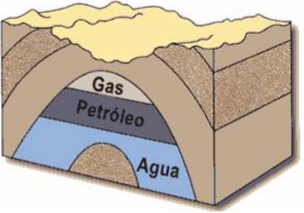
\includegraphics[scale=0.6]{images/yacimiento.png}
\caption{Diagrama transversal de una parcela. Se puede ver el reservorio correspondiente al yacimiento. Notar que dado que el agua, el gas y el petroleo tienen diferentes densidades, se forman diferentes capas.}
\end{figure}

En cada parcela puede excavarse a lo sumo un único pozo. Una vez finalizado el mismo, el producto sale a la superficie solamente a partir de la diferencia de presión entre el yacimiento y la superficie. Toda parcela tiene una determinada presión inicial de boca de pozo, que denominaremos $P_{bc,t_0}$. La profundidad desde la superficie de una parcela al yacimiento puede diferir entre parcelas.

Para perforar un pozo, es necesaria la utilización de equipos de excavación denominados RIGS, que son sumamente complejos y costosos. El costo de alquiler de los mismos depende de su poder de excavación diaria (en metros/día). Su costo de alquiler diario varia y una vez alquilada existe un mínimo de días que se debe pagar por la maquina, sea o no utilizada. En un día, solo un RIG puede ser utilizado para excavar un pozo. Además, cada modelo de RIG tiene un consumo de combustible (litros/día) al ser utilizado.

La excavación diaria de los RIGS naturalmente se ve afectada por el tipo de terreno de cada parcela. En general, existen tres tipos de suelo en un yacimiento:
\begin{enumerate}
\item Normal
\item Rocoso: Genera una resistencia a la maquina de un 60\%.
\item Arcilloso: La maquina puede ir hasta un 10\% más rápido.
\end{enumerate}

Una vez finalizado el poso, el producto puede comenzar a ser extraído si se habilita la su respectiva válvula principal. La cantidad potencial de producto ($m^3$) que puede extraerse de un pozo en un día sigue la siguiente formula:

\begin{equation} \label{eq:pressure}
PotencialVolumen_{diario \times pozo} = \alpha_1 \Bigg(\frac{P_{bc, t_i}}{N_{pozos \; habilitados}}\Bigg) +  \alpha_2 \Bigg(\frac{P_{bc, t_i}}{N_{pozos \; habilitados}}\Bigg)^2
\end{equation}

donde los rangos sugeridos son: $\alpha_1 \in [0.1 \frac{m^3}{PSIA}, \ldots, 0.6 \frac{m^3}{PSIA}]$ y $\alpha_2 \in [0.01 \frac{m^3}{PSIA}, \ldots, 0.05\frac{m^3}{PSIA}]$.

Cada día los ingenieros deben decidir si se extrae o no producto de cada pozo, abriendo o cerrando la respectiva válvula. Habilitar todos los pozos al mismo tiempo puede no ser conveniente, dado que la presión general baja por cada pozo adicional en uso, extendiendo el tiempo requerido para extraer una determinada cantidad de producto. Por otro lado, el trade off de usar menos pozos es que la velocidad de extracción también puede bajar, por lo que los ingenieros deben determinar la cantidad de pozos óptima a habilitar.

\pagebreak

Luego de que se extrajese producto de uno o mas pozos, la presión de cada uno disminuye siguiendo la siguiente formula:

\begin{equation}
P_{bc, t_{i+1}} = P_{bc, t_i} e^{-\beta_i}
\end{equation}

Es decir, la presión en boca de pozo en el día $t+1$ depende de la presión en el día $t$ de forma exponencial en un parámetro $\beta$. Este parámetro depende del periodo $i$ y se define como:

\begin{equation}
\beta_i = \frac{0.1 \times \Big(\frac{Vol_{R_i}}{Vol_R}\Big)}{\sqrt[3]{(N_{pozos})^2}}
\end{equation}

donde el $Vol_R$ es el volumen total de producto existente en el reservorio antes de su explotación (en general $Vol_R \in [10^7m^3, \ldots, 10^9m^3]$) y $Vol_{R_i}$ es el volumen total de producto en el reservorio que va quedando luego de $i$ días de explotación. Debido a que la ecuación (2) es una sucesión no constante, necesitamos un valor inicial de presión cuando comienza la vida de producción del pozo, que denominaremos $P_{bc,t_0}$. Esta presión es fija, depende de cada pozo en particular, y en general satisface que $P_{bc,t_0} \in [3000 \; PSIA, \ldots, 3500 \; PSIA]$. Resumiendo, cada día que se extrae producto, la presión de cada pozo y la cantidad potencial de $m^3$ extraíbles disminuyen.

Al abrir la válvula de un pozo (es importante mencionar que no pueden ser abiertas el mismo día en el que se finalizo su construcción), el producto extraído debe ser enviado a una planta separadora de producto. Las mismas se encargan de separar los $m^3$ recibidos en agua, gas y petroleo. Su construcción lleva una determinada cantidad de días (usualmente meses), tiene un costo y tienen una capacidad de separación dada en $m^3$. Como todos los pozos están construidos con este tipo de plantas, la cantidad de producto extraíble esta acotada por la capacidad total de separación de las plantas disponibles.

Una vez separado el producto, el petroleo no se almacena. Las refinerías se conectan directamente a través de oleoductos a las destilerías que se encargan de su refinamiento y venta. Dado que los oleoductos y las refinerías ya están disponibles, nos abstraemos de su modelado y consideramos que enviar el petroleo a una destilería es equivalente a venderlo por cierto precio.

Por otro lado, los $m^3$ de agua y el gas deben ser almacenados en tanques de almacenamiento. Los tanques tienen un costo y tiempo de construcción asociados, con una capacidad acotada. El gas almacenado en estos tanques puede venderse por cierto monto de dinero por $m^3$, dejando el espacio disponible para poder seguir almacenando gas. El volumen disponible en estos tanques puede limitar la extracción de producto.

Al pasar el tiempo, es posible que los niveles de extracción y presión empiecen a caer a niveles que no son aceptables. Estos valores son medidos por las válvulas de cada pozo de forma continua. Para mejorar la presión de los pozos y aumentar la extracción, es posible reinyectar en los pozos agua especialmente comprada y traída con camiones hidrantes, o utilizando el agua y gas almacenados en los tanques. Existe un valor de presión critica que indica cuando comienza a ser conveniente una reinyección. Al reinyectar, se recalcula el valor inicial que determina la evolución de la presión en la ecuación \ref{eq:pressure}. Este valor se recalcula utilizando la siguiente formula:

\begin{equation}
P_{bc, reinyecion_{t_0}} = P_{bc, t_0} \times \frac{Vol_R - Vol_{GlobalExtraido} + Vol_{GlobalReinyectado}}{Vol_R}
\end{equation}

donde se debe cumplir que $Vol_{GlobalReinyectado} < Vol_{GlobalExtraido}$ con el volumen global reinyectado siendo la suma del volumen de agua o gas que se reinyecta en todos los pozos que participan o participaron alguna vez de una reinyección, y volumen global extraído el volumen total histórico que se extrajo del reservorio. Cuando se reinyecta con al menos un pozo, ningún otro pozo puede extraer ese día. 

Se debe tener en cuenta que una reinyección cambia la composición del reservorio, es decir, la concentración de petroleo, gas y agua. Por esta razón, luego de una reinyección se deben recalcular estas concentraciones en función de los porcentajes antes de reinyectar $(\%Pe_i, \%Gas_i, \%Agua_i)$ con las siguientes formulas:

\begin{equation}
\%Pe_f = \frac{\%Pe_i \times (Vol_R - Vol_{GlobalExtraido})}{Vol_R - Vol_{GlobalExtraido} + Vol_{GlobalReinyectado}}
\end{equation}

\begin{equation}
\%Gas_f = \frac{\%Gas_i \times (Vol_R - Vol_{GlobalExtraido}) + Vol_{GasReinyectado}}{Vol_R - Vol_{GlobalExtraido} + Vol_{GlobalReinyectado}}
\end{equation}

\begin{equation}
\%Agua_f = \frac{\%Gas_i \times (Vol_R - Vol_{GlobalExtraido}) + Vol_{AguaReinyectada}}{Vol_R - Vol_{GlobalExtraido} + Vol_{GlobalReinyectado}}
\end{equation}

\pagebreak

El proceso de reinyección no puede hacerse de forma indefinida. Cuando el nivel de petroleo baja de determinado valor critico (dilución critica), la separación se hace muy compleja y costosa, por lo que el reservorio deja de ser rentable con los métodos de extracción actuales. Este valor critico es un parámetro de simulación, pero típicamente es un 35\% de petroleo.

Todas estas decisiones son tomadas por el equipo de ingeniería. En lineas generales, el mismo se encarga de:

\begin{enumerate}
\item Determinar en que parcelas del yacimiento se harán las perforaciones. Esta decisión en general es en función de la distancia al reservorio, el tipo de terreno, la presión inicial y otros factores.
\item Determinar en que momento se excavan los pozos, el numero de RIGS a utilizar de forma simultanea y el momento en que se construyan las diferentes plantas y tanques. Por ejemplo, un ingeniero podría decidir hacer todos los pozos lo antes posible utilizando la máxima cantidad de RIGS de forma simultanea, o construirlos en orden ascendente de dificultad. En cuanto a la construcción de las plantas/tanques, pueden ser construidos a medida que son necesarios o planificando a futuro dependiendo de cuanto se espera producir.
\item Decidir cuantos pozos de los disponibles se usan para extraer producto día a día. Por ejemplo, se pueden utilizar todos los disponibles o los que tengan mayor presión en un día dado.
\item Determinar cuando reinyectar y cuanto. Cuando se llega a la presión critica de un pozo se puede reinyectar todo lo que se posea de agua y gas almacenado hasta que se alcance un valor de presión esperado, o solo se puede reinyectar agua (comprando de ser necesario) y el gas se vende de la misma forma que el petroleo.
\item Decidir cuando el yacimiento deja de ser rentable y se termina de extraer producto. Por ejemplo, se puede decidir que ya no vale la pena seguir extrayendo petroleo cuando se llega a una dilución critica de 35\% de petroleo. 
\end{enumerate}

Tomando en cuenta todos estos factores, el simulador debe funcionar a partir de los siguientes parámetros de simulación:
\begin{enumerate}
\item Tamaño del yacimiento.
\item Cantidad de pozos que se quieren realizar en el yacimiento.
\item Cantidad máxima de RIGS a utilizarse en simultaneo.
\item Presión critica de los pozos, valor a partir del cual es conveniente reinyectar.
\item Dilución critica del reservorio.
\item Costos de cada factor.
\end{enumerate}

El simulador también debe reportar en un Log todo lo que se debería efectuar día a día en el yacimiento, el costo total del emprendimiento, el dinero total vendido de gas y petroleo y la ganancia resultante.

\begin{figure}[H]
    \centering
    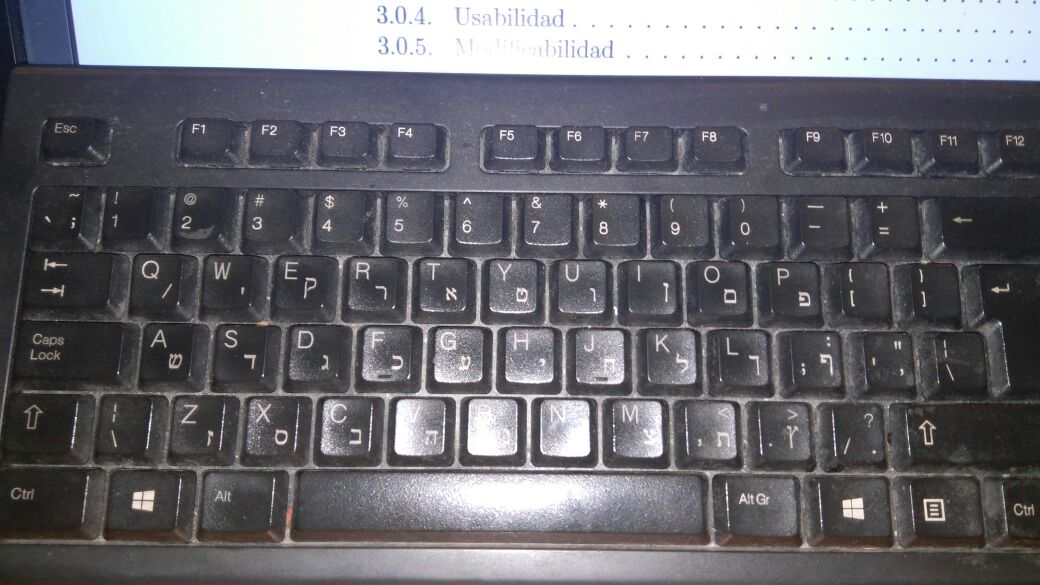
\includegraphics[scale=0.3]{images/teclado.jpeg}
    \caption{Scrum Master dando ordenes desde un hotel en Israel.}
\end{figure}

\pagebreak

\section{Requerimientos funcionales}

\subsection{User Stories}
El Product Owner de nuestro equipo (cuya identidad no revelaremos) ha trabajado en conjunto con los desarrolladores y los expertos de dominio para construir un Product Backlog constituido por los siguientes user stories. Los Story Points son una medida utilizada comúnmente por los equipos de SCRUM para dar cuantificar el tiempo requerido de implementación. Luego, el Business Value busca cuantificar el valor que un User Story especifico aporta al proyecto en general.

\subsubsection{Representación de un yacimiento}
    Iniciamos por el paso mas básico que es el de representar el elemento central de la simulación, el yacimiento:\\
    
    \fcolorbox{gray}{white}{
      \parbox{0.9\textwidth}{
        Como \textbf{Empleado del ministerio} quiero \textbf{ingresar la composición inicial del yacimiento a simular} para \textbf{reflejar un yacimiento real a licitar en el simulador}
      }
    }\\
    
    \textbf{Story points: 1}
    
    \textbf{Business Value: 5}


\subsubsection{Construcción de un mapa}
    Luego queremos representar el terreno donde se realizara la actividad de ese yacimiento:\\
    
    \fcolorbox{gray}{white}{
      \parbox{0.9\textwidth}{
        Como \textbf{Empleado del Ministerio} quiero \textbf{generar un mapa de parcelas, con sus profundidades, tipos de suelo, presiones iniciales y pozos ya realizados} para \textbf{reflejar un terreno real a licitar}
      }
    }\\
    
    \textbf{Story points: 2}
    
    \textbf{Business Value: 6}

\subsubsection{Cotizar materia prima}
    Ahora queremos modelar los valores de mercado de lo extraido:\\
    
    \fcolorbox{gray}{white}{
      \parbox{0.9\textwidth}{
        Como \textbf{Empleado del ministerio} quiero \textbf{ingresar cotizaciones de materias primas} para \textbf{que las ganancias resultantes concuerden con la realidad}
      }
    }\\
    
    \textbf{Story points: 1}
    
    \textbf{Business Value: 2}

\subsubsection{Extracción}
    Necesitamos que se extraiga lo que sea necesario y posible de un pozo especifico

    \fcolorbox{gray}{white}{
      \parbox{0.9\textwidth}{
        Como \textbf{Ingeniero} quiero \textbf{decidir cuanto extraer de un pozo} para \textbf{generar ganancias}
      }
    }\\
    
    \textbf{Story points: 2}
    
    \textbf{Business Value: 2}

\subsubsection{Simular un día}
    Para tener una versión inicial del sistema, se quiere lograr primero una simulación simple para decidir si se esta yendo por un buen camino:\\
    
    \fcolorbox{gray}{white}{
      \parbox{0.9\textwidth}{
        Como \textbf{Empleado del ministerio} quiero \textbf{simular el paso de un día} para \textbf{tener una vista inicial del simulador}
      }
    }\\
    
    \textbf{Story points: 4}
    
    \textbf{Business Value: 4}
    
\subsubsection{Excavación de un nuevo pozo}
    Es clave que se simule el alquiler de un RIG para excavar pozos nuevos en las parcelas:\\
    
    \fcolorbox{gray}{white}{
      \parbox{0.9\textwidth}{
        Como \textbf{Empleado del Ministerio} quiero \textbf{que se puedan crear nuevos pozos} para \textbf{aprovechar el yacimiento mas ampliamente}
      }
    }\\
    
    \textbf{Story points: 3}
    
    \textbf{Business Value: 4}\\
    
    \fcolorbox{gray}{white}{
      \parbox{0.9\textwidth}{
        Como \textbf{Ingeniero} quiero \textbf{decidir si alquilar un RIG} para \textbf{poder utilizarlo en la excavación de un pozo nuevo}
      }
    }\\
    
    \textbf{Story points: 1}
    
    \textbf{Business Value: 2}\\
    
    \fcolorbox{gray}{white}{
      \parbox{0.9\textwidth}{
        Como \textbf{Ingeniero} quiero \textbf{utilizar un RIG para iniciar la excavación de un nuevo pozo} para \textbf{luego poder extraer recursos de el}
      }
    }\\
    
    \textbf{Story points: 3}
    
    \textbf{Business Value: 3} 

\subsubsection{Infraestructura}
    Necesitamos que haya plantas separadoras para poder utilizar la materia prima extraída y/o almacenarla\\
    
    \fcolorbox{gray}{white}{
      \parbox{0.9\textwidth}{
        Como \textbf{Empleado del ministerio} quiero \textbf{que haya plantas separadoras} para \textbf{poder utilizar las distintas materias primas en la simulación}
      }
    }\\
    
    \textbf{Story points: 2}
    
    \textbf{Business Value: 2}\\
    
    También necesitamos tanques de agua y gas:\\
    
    \fcolorbox{gray}{white}{
      \parbox{0.9\textwidth}{
        Como \textbf{Empleado del ministerio} quiero \textbf{que haya tanques de agua y gas} para \textbf{almacenar el agua y gas extraídos}
      }
    }\\
    
    \textbf{Story points: 2}
    
    \textbf{Business Value: 2} 

\subsubsection{Reinyección}
    Una parte esencial es simular la reinyección de agua o gas a un pozo para aumentar la presión de su boca:\\
    
    \fcolorbox{gray}{white}{
      \parbox{0.9\textwidth}{
        Como \textbf{Empleado del Ministerio} quiero \textbf{que se reinyecte gas o agua} para \textbf{aumentar la presión en la boca de pozo}
      }
    }\\
    
    \textbf{Story points: 2}
    
    \textbf{Business Value: 3}\\

    \fcolorbox{gray}{white}{
      \parbox{0.9\textwidth}{
        Como \textbf{Empleado del Ministerio} quiero \textbf{poder limitar hasta que valor de dilución es rentable reinyectar} para \textbf{no estar desperdiciando recursos en este punto de la simulación}
      }
    }\\
    
    \textbf{Story points: 1}
    
    \textbf{Business Value: 2}

\subsubsection{Políticas}
    Ahora queremos poder elegir políticas que van a utilizar el equipo de ingenieros a simular para tomar decisiones de excavación, construcción, equipamiento, y distribución:\\
    
    \fcolorbox{gray}{white}{
      \parbox{0.9\textwidth}{
        Como \textbf{Empleado del Ministerio} quiero \textbf{ver las políticas disponibles de excavación, construcción, equipamiento, y distribución} para \textbf{poder elegir correctamente cada una}
      }
    }\\
    
    \textbf{Story points: 1}
    
    \textbf{Business Value: 2}\\

    \fcolorbox{gray}{white}{
      \parbox{0.9\textwidth}{
        Como \textbf{Empleado del Ministerio} quiero \textbf{elegir las políticas de excavación, construcción, equipamiento, y distribución} para \textbf{buscar la combinación que produzca mas ganancia}
      }
    }\\
    
    \textbf{Story points: 2}
    
    \textbf{Business Value: 3}\\
    
    \fcolorbox{gray}{white}{
      \parbox{0.9\textwidth}{
        Como \textbf{Ingeniero} quiero \textbf{elegir que pozos excavar y reinyectar en base a una política de excavación} para \textbf{obtener mas materia prima}
      }
    }\\
    
    \textbf{Story points: 2}
    
    \textbf{Business Value: 2}\\
    
    \fcolorbox{gray}{white}{
      \parbox{0.9\textwidth}{
        Como \textbf{Ingeniero} quiero \textbf{cuando construir infraestructura} para \textbf{no estar limitado por la infraestructura actual}
      }
    }\\
    
    \textbf{Story points: 2}
    
    \textbf{Business Value: 2}\\
    
    \fcolorbox{gray}{white}{
      \parbox{0.9\textwidth}{
        Como \textbf{Ingeniero} quiero \textbf{alquilar nuevo equipo en base a una política de equipamiento} para \textbf{tener equipo disponible para nuevas tareas}
      }
    }\\
    
    \textbf{Story points: 1}
    
    \textbf{Business Value: 2}\\
    
    \fcolorbox{gray}{white}{
      \parbox{0.9\textwidth}{
        Como \textbf{Ingeniero} quiero \textbf{decidir donde enviar la materia prima} para \textbf{venderla o reutilizarla y que no quede ociosa}
      }
    }\\
    
    \textbf{Story points: 2}
    
    \textbf{Business Value: 3}

\subsubsection{Simulación extendida en el tiempo}
    En este punto ya queremos simular el paso de tiempo a largo plazo, ya que hay procesos que llevan tiempo y un día no puede reflejarnos todo:\\
    
    \fcolorbox{gray}{white}{
      \parbox{0.9\textwidth}{
        Como \textbf{Empleado del Ministerio} quiero \textbf{simular a largo plazo} para \textbf{reflejar el ciclo de vida real de un yacimiento}
      }
    }\\
    
    \textbf{Story points: 6}
    
    \textbf{Business Value: 5}

\subsubsection{Registro}
    Queremos que se registren todas las acciones tomadas por el equipo de ingeniería y las realizadas en cada dia simulado, registrando la accion y el costo o ganancia segun corresponda:\\
    
    \fcolorbox{gray}{white}{
      \parbox{0.9\textwidth}{
        Como \textbf{Empleado del Ministerio} quiero \textbf{acceder a un registro de actividades de la simulación} para \textbf{analizar la evolución del ciclo de vida del yacimiento}
      }
    }\\
    
    \textbf{Story points: 2}
    
    \textbf{Business Value: 4}\\
    
    \fcolorbox{gray}{white}{
      \parbox{0.9\textwidth}{
        Como \textbf{Empleado del Ministerio} quiero \textbf{acceder a un registro de contaduría de la simulación} para \textbf{analizar la ganancia real de la explotación ejecutada}
      }
    }\\
    
    \textbf{Story points: 2}
    
    \textbf{Business Value: 5}
    
\subsubsection{Pozos a realizar y RIGs a alquilar}
    Como fue requerido, queremos poder limitar la cantidad de pozos que se pueden construir y RIGs que se pueden alquilar:\\
    
    \fcolorbox{gray}{white}{
      \parbox{0.9\textwidth}{
        Como \textbf{Empleado del ministerio} quiero \textbf{elegir cuantos pozos se van a construir como máximo} para \textbf{poder probar que cantidad genera mas ganancia}
      }
    }\\
    
    \textbf{Story points: 1}
    
    \textbf{Business Value: 1}\\
    
    \fcolorbox{gray}{white}{
      \parbox{0.9\textwidth}{
        Como \textbf{Empleado del ministerio} quiero \textbf{elegir cuantos RIGs se van a alquilar como máximo} para \textbf{poder probar que cantidad genera mas ganancia}
      }
    }\\
    
    \textbf{Story points: 1}
    
    \textbf{Business Value: 1} 
 
\subsubsection{Finalización de simulación}
    Queremos que se pueda decir cuando detener la simulación:\\
    
    \fcolorbox{gray}{white}{
      \parbox{0.9\textwidth}{
        Como \textbf{Empleado del ministerio} quiero \textbf{definir la condición que dará por finalizada la simulación sobre el terreno} para \textbf{controlar los tiempos de simulación}
      }
    }\\
    
    \textbf{Story points: 2}
    
    \textbf{Business Value: 3}

\subsubsection{Extensión de estrategias}
    Finalmente queremos que se pueda extender la lista acotada de estrategias posibles de excavación, distribución, construcción y equipamiento:\\
    
    \fcolorbox{gray}{white}{
      \parbox{0.9\textwidth}{
        Como \textbf{Empleado del ministerio} quiero \textbf{agregar estrategias de excavación, distribución, construcción y equipamiento} para \textbf{definir nuevos patrones de excavación, distribución, construcción y equipamiento respectivamente}
      }
    }\\
    
    \textbf{Story points: 2}
    
    \textbf{Business Value: 3}
    

\subsection{Extendiendo algunos user stories}

En esta sección seleccionaremos los tres user stores que consideramos mas relevantes, los describiremos en detalle y haremos su respectiva descomposición en tareas, estimando el tiempo de RRHH necesario para su implementación y definiendo diferentes criterios de aceptación.

\subsubsection{User Storie \#1}
\begin{framed}
 Como \textbf{Empleado del Ministerio} quiero \textbf{generar un mapa de parcelas, con sus profundidades, tipos de suelo, presiones iniciales y pozos ya realizados} para \textbf{reflejar un terreno real a licitar}
\end{framed}

\subsubsection*{Descomposición en tareas}

\begin{enumerate}
  \item Crear subclases de Tipo de terreno que representen los suelos posibles.
  \item Crear la clase EstadoDeParcela y sus sublclases Perforada y SinPerforar, para representar parcelas con pozos ya realizados.
  \item Crear la clase Parcela y su método de inicialización que reciba el tipo de terreno, profundidad, presión inicial y su estado.
  \item Crear la clase MapaDeParcelas con su método de inicialización que reciba una colección de parcelas.
\end{enumerate}

\subsubsection*{Estimación de RRHH necesarios}

Dos desarrolladores Junior, ya que son clases bastante básicas en esta iteración.

\subsubsection*{Criterios de aceptación}

Se pueden inicializar parcelas con los parámetros dichos antes, almacenarlas en una colección y utilizarlas para inicializar un Mapa de Parcelas.

\subsubsection{User Storie \#2}
\begin{framed}
  Como \textbf{Empleado del Ministerio} quiero \textbf{simular a largo plazo} para \textbf{reflejar el ciclo de vida real de un yacimiento}
\end{framed}

\subsubsection*{Descomposición en tareas}

\begin{enumerate}
  \item Crear la clase Calendario que pueda inicializarse en una fecha y pueda avanzar de día.
  \item Modificar la clase EscenarioDeSimulación para que inicialice un calendario al inicializarce.
  \item Implementar método simularHastaCondiciónDeFin en la clase EscenarioDeSimulación que reciba un closure que represente la condición y reciba el escenario de simulación. Que simule y avance el calendario hasta que se cumpla esa condición.
\end{enumerate}

\subsubsection*{Estimación de RRHH necesarios}

Un desarrollador Junior y uno SSr, ya que para lograr algo no tan acoplado debería haber alguien con experiencia que sepa sobre DOO.

\subsubsection*{Criterios de aceptación}

Se puede crear un closure que por ejemplo devuelva true pasados 20 días de simulación. Que se le pueda enviar el mensaje simularHastaCondiciónDeFin con este closure y el Simulador simule día por día hasta que el closure devuelva true, osea hasta el día 20.

\subsubsection{User Storie \#3}
\begin{framed}
  Como \textbf{Empleado del Ministerio} quiero \textbf{acceder a un registro de contaduría de la simulación} para \textbf{analizar la ganancia real de la explotación ejecutada}
\end{framed}

\subsubsection*{Descomposición en tareas}

\begin{enumerate}
  \item Crear la clase RegistroDeContaduria que se inicialice con un calendario y pueda registrar gastos y ganancias, y responder los gastos y ganancia total de un día especifico.
  \item Modificar la clase EscenarioDeSimulación para que inicialice un registro y lo responda cuando se lo piden.
  \item Modificar la clase Simulador para que le pida el registro al EscenarioDeSimulacion
  \item Modificar la clase AdministradorFinanciero para que registre cada gasto y ganancia en el RegistroDeContaduria que le puede pedir al Simulador
  \item Modificar la InterfazDeSimulador para que al responder mostrarActividades también informe las cuentas de esas actividades.
\end{enumerate}

\subsubsection*{Estimación de RRHH necesarios}

Dos desarrollador Junior y uno Sr., ya que necesitamos alguien con experiencia que sepa como organizar estas clases sin que se acoplen, y como son varias tareas a hacer es mejor tener mas personal.

\subsubsection*{Criterios de aceptación}

Luego de simular correctamente, se pueda enviar el mensaje mostrarActividades a la InterfazDeSimulador y que muestre en un transcript las acciones realizadas cada día y los gastos y ganancias totales de cada día.

\pagebreak

\section{Diseño}

Para este Tp se intento desarrollar una diseño lo mas extensible posible. Es decir que tuviera buenos ejes de cambio, y poco acoplamiento, apelando a los principios de diseño visto en clase, tratando de ser lo mas cohesivo posible en cada clase. Nos encontramos con que las formulas del enunciado no limitaron mucho con respecto a la relacion de conociminto entre los objetos. Se intento apelar al uso de subclasificacion y estate pattern para evitar el uso IFs innecesarios en base a polimorfismo.

\subsection{Diagramas de objetos}

\begin{figure}[H]
\centerline{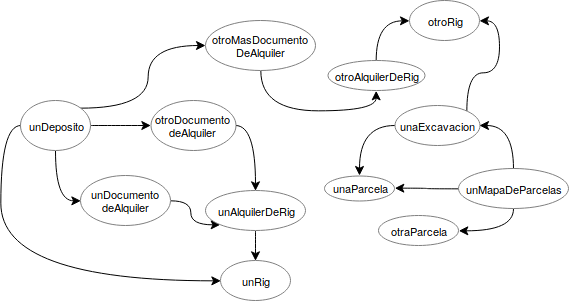
\includegraphics[scale=0.5]{images/DiagramaDeObjetos_deRigs.png}}
\caption{Diagrama de objetos de RIGs}
\end{figure}

Aquí podemos ver como varia la relación de conocimiento con respecto al RIG. Lo que queremos exhibir aquí un deposito puede conocer un documento de alquiler y un alquiler de un RIG que no necesariamente esta actualmente depositado en el deposito. La razón de esto es porque ese RIG se retiro de allí para ponerlo a excavar. En consecuencia, ya no puede estar disponible en el deposito para otra nueva excavación hasta que la excavación actual que utiliza ese RIG termine. No obstante la relación de conocimiento entre el deposito y el alquiler no se pierde por retirar un RIG, si no que esta se pierde cuando explícitamente se decide cancelar dicho documento. De esta forma se puede calcular el costo de todos los alquileres mas allá de que el RIG este depositado o no actualmente en el deposito.

\begin{figure}[H]
\centerline{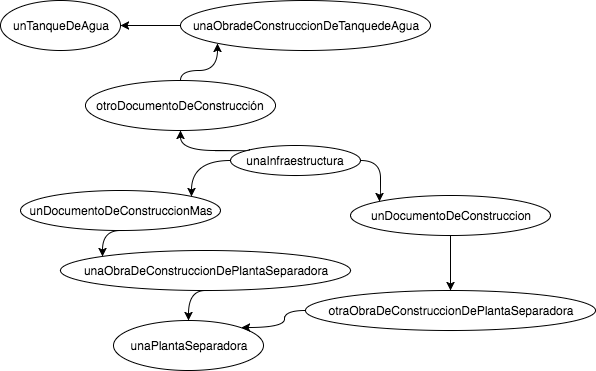
\includegraphics[scale=0.4]{images/DiagramaDeObjetosDeObrasDeContruccion.png}}
\caption{Diagrama de objetos de obras de construcción}
\end{figure}

Acá podemos ver como puede haber casos en el que haya dos potenciales obras a realizar para construir una misma construcción (dos ofertas diferentes, de dinero y/o plazos) como podemos ver para construir una planta separadora en este diagrama. Y claramente también hay otros casos en el que hay una sola oferta de obra, como en este caso podemos ver para la construcción de un tanque de agua. En el caso de varias obras posibles a realizar, el Directorio de Ingeniería, siguiendo la política de construcción elegida va a llevar a cabo la obra que corresponda mas.
Cada vez que se comienza una obra de construcción en una infraestructura se crea un nuevo documento de obra de construcción del cual la infraestructura mantiene conocimiento. Dichos documentos de construcción pueden hacer referencia a obras de construcción de cualquier índole, por ejemplo de planta separadora, de tanque de agua o gas, y posibles nuevas obras de construcción.
\pagebreak

\subsection{Diagramas de clases}

\subsubsection{Simulador}

\begin{figure}[H]
\centerline{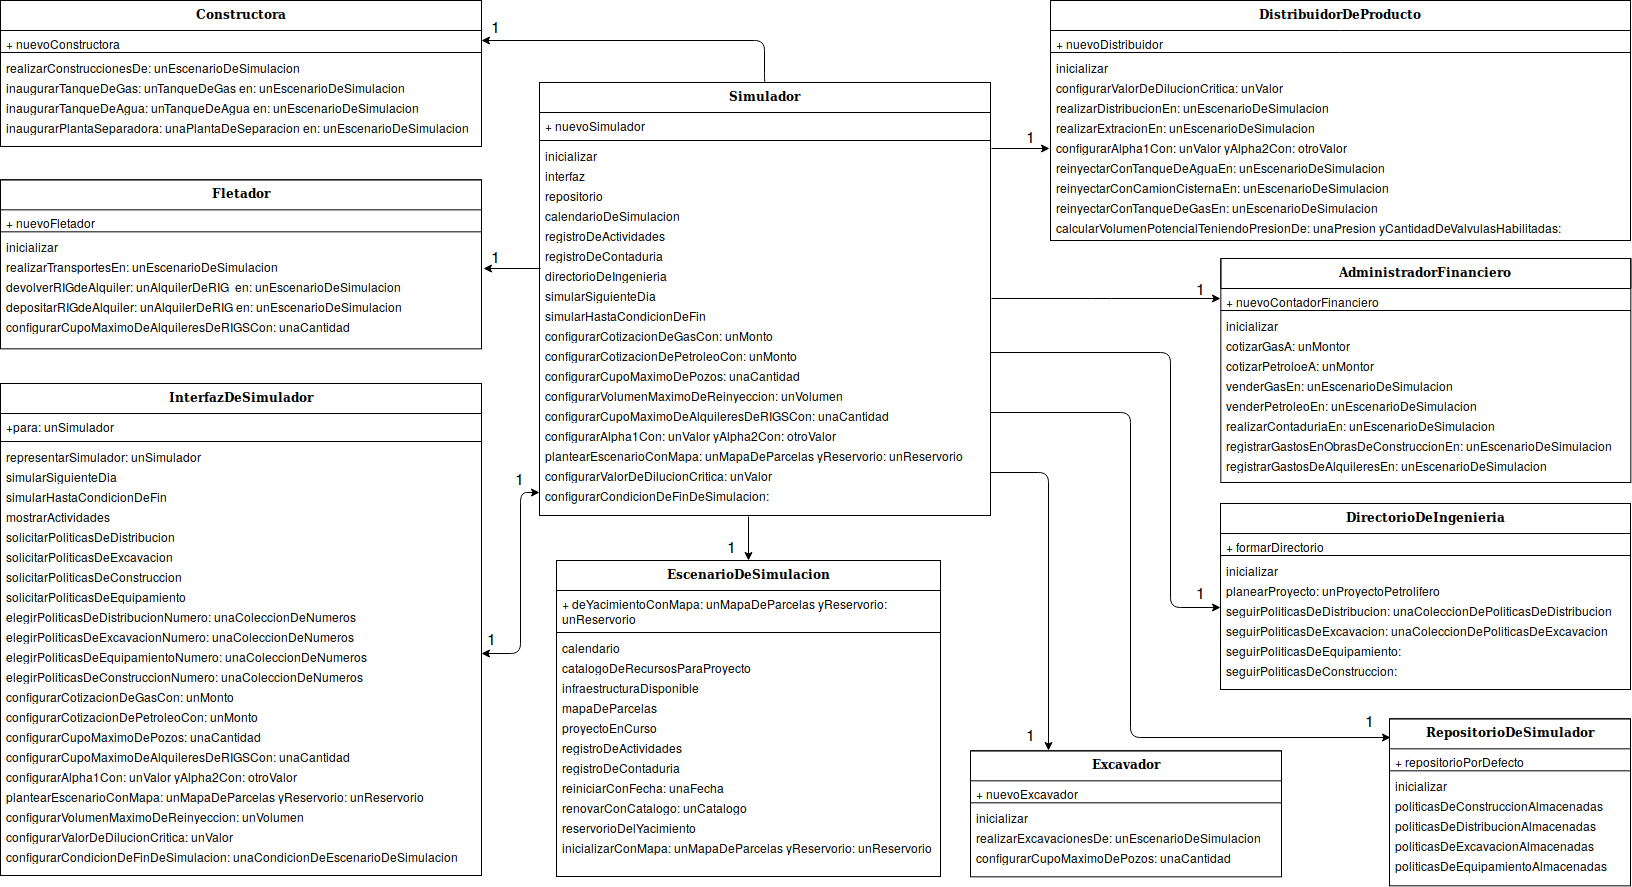
\includegraphics[scale=0.36]{images/DiagramaDeClases_deSimulador.png}}
\caption{Diagrama de clases del Simulador}
\end{figure}

El simulador tiene el rol del un orquestrador. El mismo maneja la coherencia y el orden de ejecución entre los componentes del simulador. El usuario del simulador puede interactuar con el mismo mediante la Interfaz de Simulador. Mediante la interfaz uno puede configurar todos los parámetros de la simulación, entre ellos el volumen máximo de inyección, el valor de dilución critica, el cupo máximo de alquileres de RIGs, la cantidad máxima de pozos, la cotización de petroleo y gas y la condición de fin de simulación. También nos va a dejar administrar y seleccionar las políticas a tomar por el Directorio de Ingeniería, ya sea de explotación, distribución, construcción y equipamiento, que se almacenan en un Repositorio del Simulador, pero veremos mas específicamente esto luego.

Este diagrama es esencial para entender la arquitectura general del simulador. Muchos conceptos los definiremos brevemente a continuación y luego los explicaremos mas en detalle en las correspondientes subsecciones.

En el simulador discretizamos el tiempo en días. El escenario representa un instante especifico del yacimiento en el que se encuentra el simulador, el estado de la materia prima y el estado geográfico. El mismo va mutando a medida que los distintos componentes del simulador van interactuando con el mismo. 

El encargado de decidir que acciones tomar en el yacimiento es el Directorio de Ingeniería, que usando las políticas elegidas y los recursos disponibles va a tomar decisiones validas a realizar en el escenario, lo veremos mejor luego.

Un escenario conoce un Proyecto Petrolífero, este representa los recursos disponibles y se encarga de administrar las acciones que se están realizando y que se van a realizar en el yacimiento, ya sea de explotación, distribución, construcción y equipamiento, por parte del Directorio de Ingeniería. La función principal del proyecto petrolífero es hacer la interfaz entre el Directorio de Ingeniería y el escenario de simulación.

Dado que el objetivo principal del simulador es medir el nivel de rentabilidad del mismo para luego realizar los pliegos de licitación, contamos con el Administrador Financiero que es el que se va a encargar de auditar los gastos y ganancias de las acciones tomadas en la simulación.

Algo mas que podemos ver en este diagrama es el Distribuidor de Producto, que se encarga de manejar todo lo que tiene que ver con la extracción, reinyección y distribución del producto, de la parte geológica de la explotación sabe como varían las presiones y diluciones del producto. Lo veremos mas en contexto luego.

El simulador también conoce al Excavador que es el que se va a encargar de efectivamente realizar las excavaciones requeridas, luego hablaremos mas de esto.

\subsubsection{Escenario de Simulación}

\begin{figure}[H]
\centerline{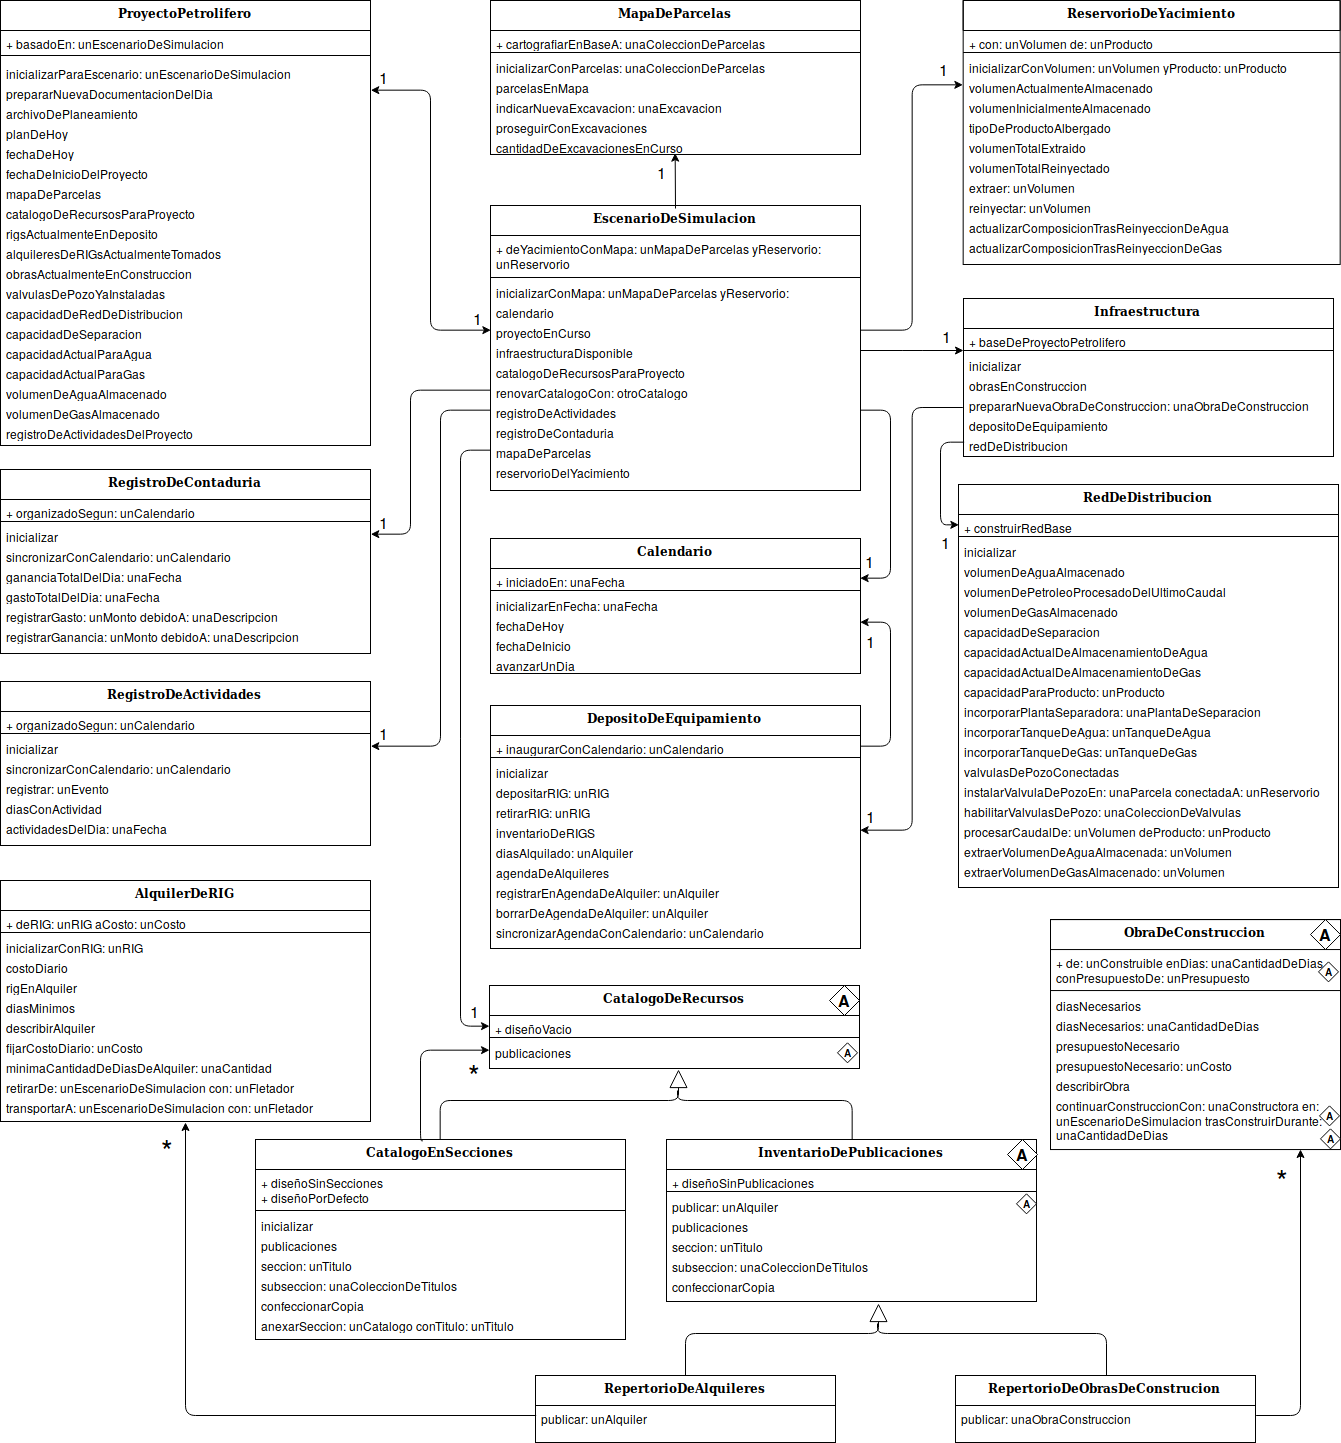
\includegraphics[scale=0.42]{images/DiagramaDeClases_deEscenario.png}}
\caption{Diagrama de clases de un Escenario de Simulación}
\end{figure}

El escenario representa el instante especifico del yacimiento en el que se encuentra el simulador. El escenario de simulación conoce el Reservorio de Yacimiento y el Mapa de Parcelas. 
El Mapa de Parcelas contiene todas las parcelas del yacimiento, como también así las excavaciones en curso.
A partir del Reservorio de Yacimiento podemos saber cual es el volumen actual que contiene y cual es la composición del mismo (compuesto por agua, gas y petroleo). El escenario de simulación también conoce el estado de la infraestructura del proyecto, que comprende al deposito de equipamiento (donde se registran y almacenan los RIGs) y a la red de distribución. La red de distribución conoce tres sub redes, la red de almacenamiento, la red de separación y la red de pozos. Las tres se utilizan para realizar modelar correctamente la distribución, extracción y reinyección. Mas adelante lo revisaremos.

El Escenario de Simulación conoce al Proyecto Petrolífero. Como dijimos antes, un Proyecto Petrolífero es la representación documentada del escenario, conoce varios datos fundamentales para la toma de decisiones por parte del Directorio de Ingeniería. Limita el conocimiento que el Directorio de Ingeniería puede tener sobre el escenario de simulación como así también define una interfaz para el mismo. 
El Escenario de Simulación también conoce la clase abstracta Catalogo que representa a los recursos disponibles para desarrollar el emprendimiento, tales como los alquileres disponibles de catalogo, las diferentes obras de tanques de agua, tanques de gas y planta separadoras que pueden ser realizadas, con sus respectivos precios. Esto lo diseñamos con un patrón Composite para conseguir la mayor extensiblidad posible. Queríamos poder subdividir el catalogo en diferentes módulos correspondientes a cada categoría de recursos. En principio podemos dividir los recursos del emprendimiento en dos categorías principales, equipamiento (Ej. maquinaria, RIGs) y obras de construcción (todos los recursos edilicios, como plantas separadoras y tanques de almacenamiento).

Algo muy importante que se puede ver en este diagrama son el Registro de Actividades y el de Contaduría, que van a mantener registradas las actividades y los gastos/ganancias respectivamente, son clave para el sistema ya que el sentido del simulador es obtener las ganancias potenciales que puede tener un yacimiento junto con un log de actividades realizadas. La forma en que se va registrando en dichos registros la detallaremos mas adelante.

Por ultimo, el escenario de simulación conoce un calendario. Este calendario se utiliza para saber el momento actual en la discretización del tiempo y en base a ello determinar cuantos días han transcurrido en la simulación. Es de vital importancia para el seguimiento de los alquileres, las obras actualmente en construcción.


\subsubsection{Red de Distribución}

\begin{figure}[H]
\centerline{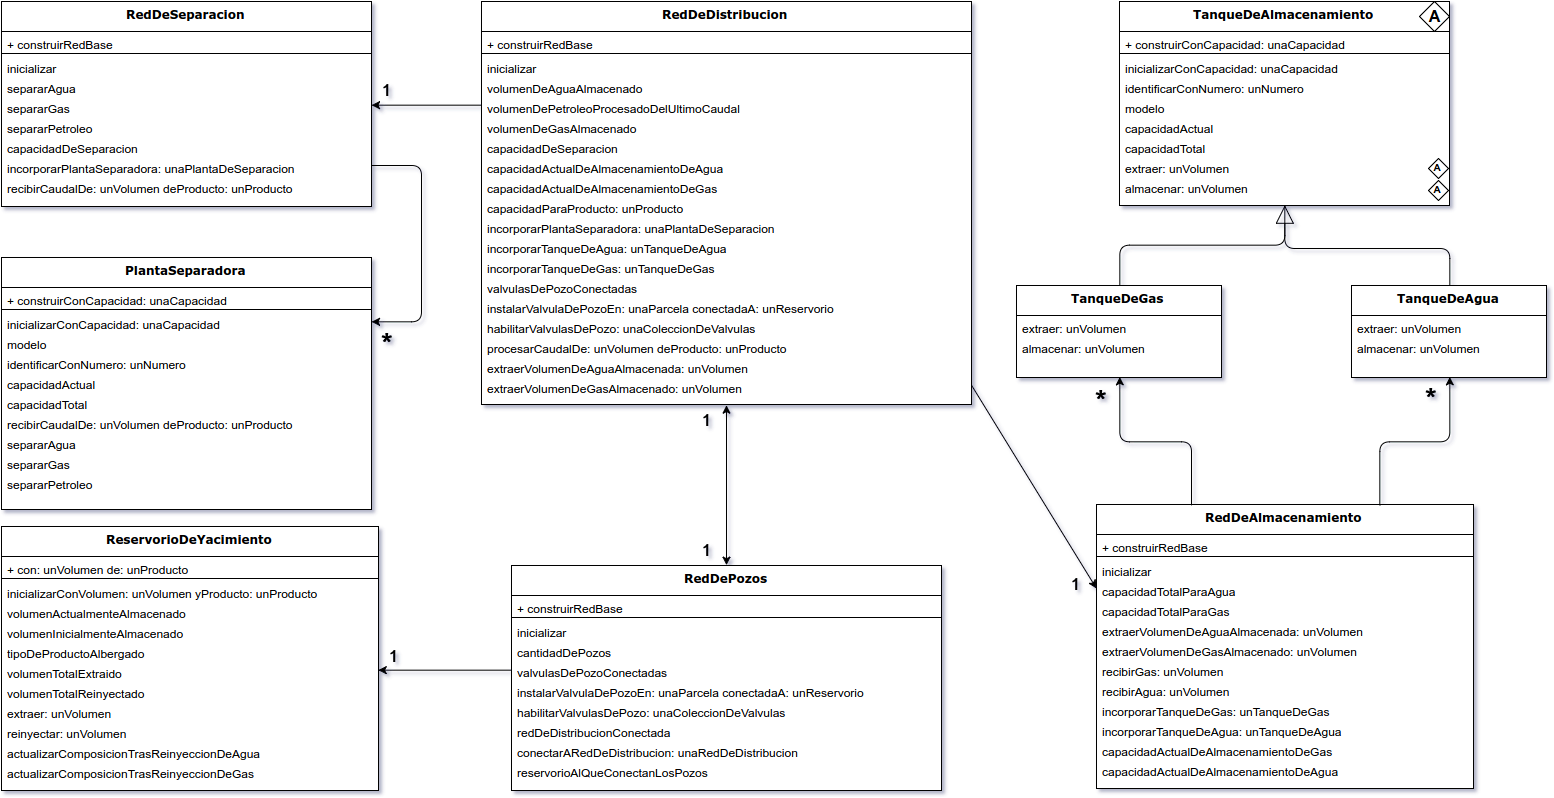
\includegraphics[scale=0.37]{images/DiagramaDeClases_deRedDeDistribucion.png}}
\caption{Diagrama de clases de la Red de Distribución}
\end{figure}

La red de distribución esta compuesta por tres subredes dedicadas con diferentes fines, la de separación de producto, la de pozos y la de almacenamiento. La red de almacenamiento es la sección de la red de distribución que se encarga de almacenar y y repartir el volumen separado en los tanques correspondiente, según sea agua o gas. Analógicamente la red de separación va incorporando plantas separadoras a medida que las mismas se terminan de construir. A la red de distribución se le puede ir incorporando los distintos diferentes plantas separadoras, tanques de gas, tanque de agua.

La red de pozos es la parte de la red de distribución que interactúa propiamente con los pozos mediante una serie de válvulas de pozo que pueden ser configuradas según el volumen y el tipo de distribución que se quiera realizar. Estas luego se habilitaran para iniciar dicha distribución configurada.

Para concluir, la Red de Distribución es la que se encarga de manejar los limites físicos que se tienen para almacenar, incorporar y eliminar las materias primas de la infraestructura.

\subsubsection{Red de Pozos}

\begin{figure}[H]
\centerline{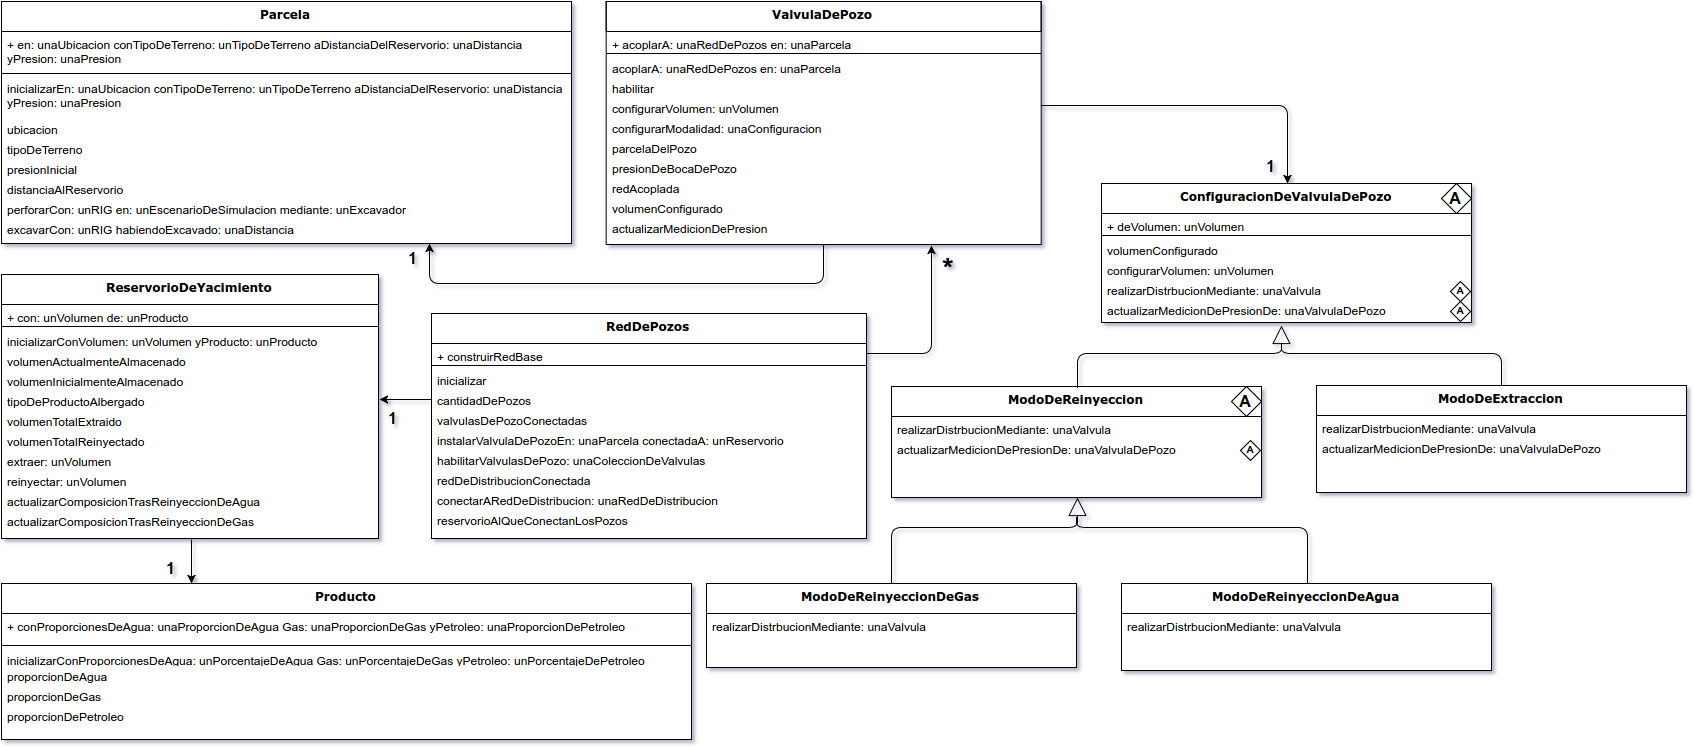
\includegraphics[scale=0.34]{images/DiagramaDeClases_deRedDePozos.png}}
\caption{Diagrama de clases de la Red de Pozos}
\end{figure}

La Red de pozo representa los pozos y la red de conexión que hay entre ellos y el resto de a red de distribución. El mismo conoce el reservorio al que desembocan las parcelas en las que se instalo una válvula de pozo. En base a estas válvulas se configura que volumen se quiere distribuir a/hacia el pozo, y en que modalidad, es decir, para extraer, reiyectar, y que tipo de reinyeccion. Vale aclarar que el reservorio además de conocer el volumen almacenado en el, conoce un Producto, que define la composición de agua, gas y petroleo del liquido almacenado allí. Es posible que el nombre Producto sea un poco ambiguo, por eso consideramos a lugar esta aclaración.


\subsubsection{Archivo de Planeamiento}

\begin{figure}[H]
\centerline{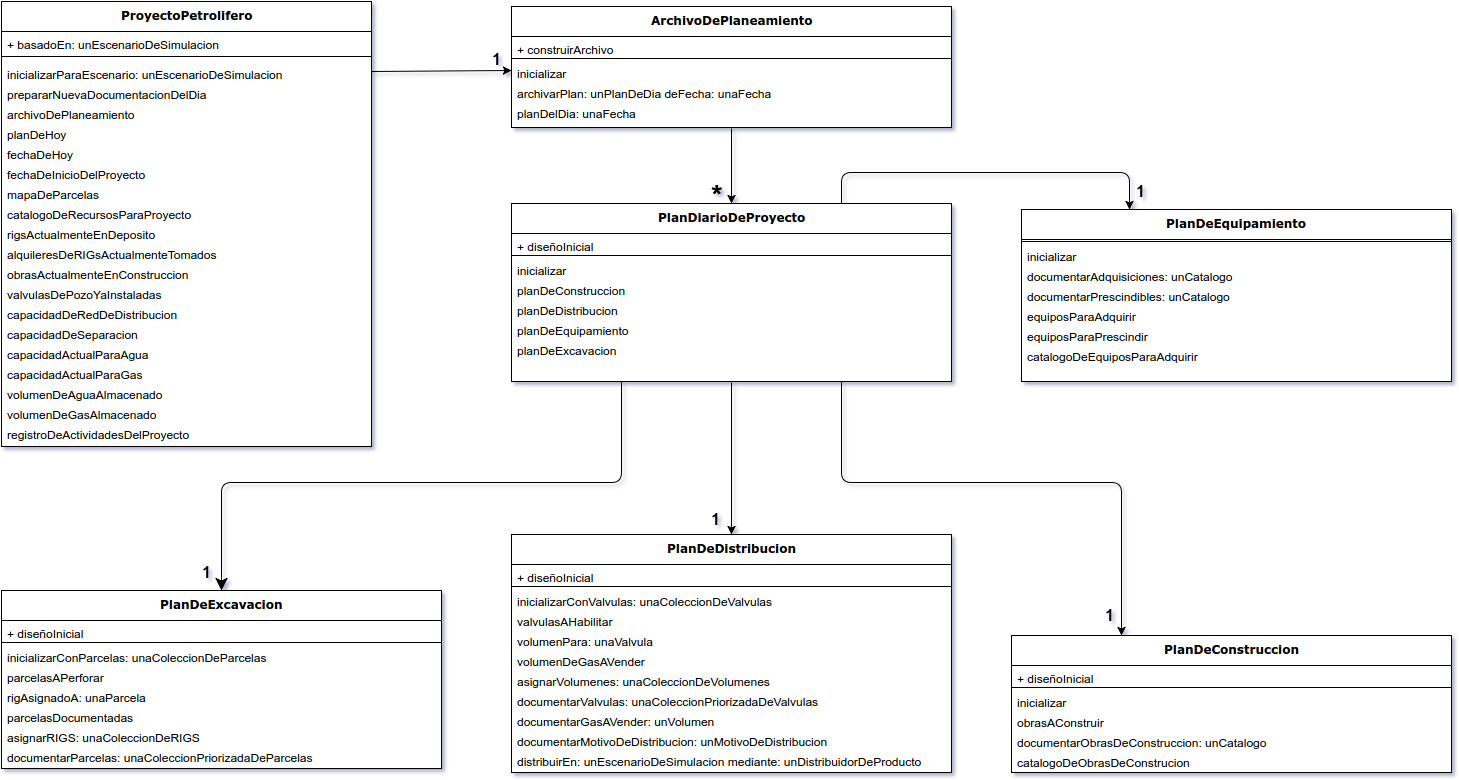
\includegraphics[scale=0.39]{images/DiagramaDeClases_ArchivoDePlaneamiento.png}}
\caption{Diagrama de clases del Archivo de Planeamiento}
\end{figure}

El Archivo de Planeamiento cumple el rol de almacenar los planes diarios del proyecto. Para esto organiza dichos planes por cada día, de manera de permite archivar u observar un plan de día en alguna fecha en particular que sea de interés. Los planes de día están a su vez subdivididos en planes mas específicos según el índole del que prediquen. En total son 4 subplanes: de construcción, de equipamiento, de excavación, y de distribución. El plan de construcción permite documentar todas las obras a construir en ese día, y el plan de de equipamiento permite documentar todos los alquileres de RIGs que se quieren empezar a alquilar, como también los que quieren dejarse de alquilar (los alquileres prescindibles). Por otro lado el plan de excavación permite documentar en que parcelas se quiere realizar nuevas excavaciones, y también con que RIGs. Ambos además son documentados con algún criterio de prioridad, de manera de que en caso de que hayamos documentado mas parcelas que una cantidad N de pozos que es posible realizar (cantidad configurado previamente desde la interfaz), se excavara en las primeras N parcelas de mayor prioridad según el criterio documentado. Análogamente el plan de distribución permite documentar las válvulas que se desean habilitar según una prioridad documentada. En el mismo también se documenta que volumen configurar a cada válvula, y que tipo de distribución se desea realizar (extracción, reinyección por tanques de agua, por tanques de gas etc).  

\subsubsection{Directorio de Ingeniería}

\begin{figure}[H]
\centerline{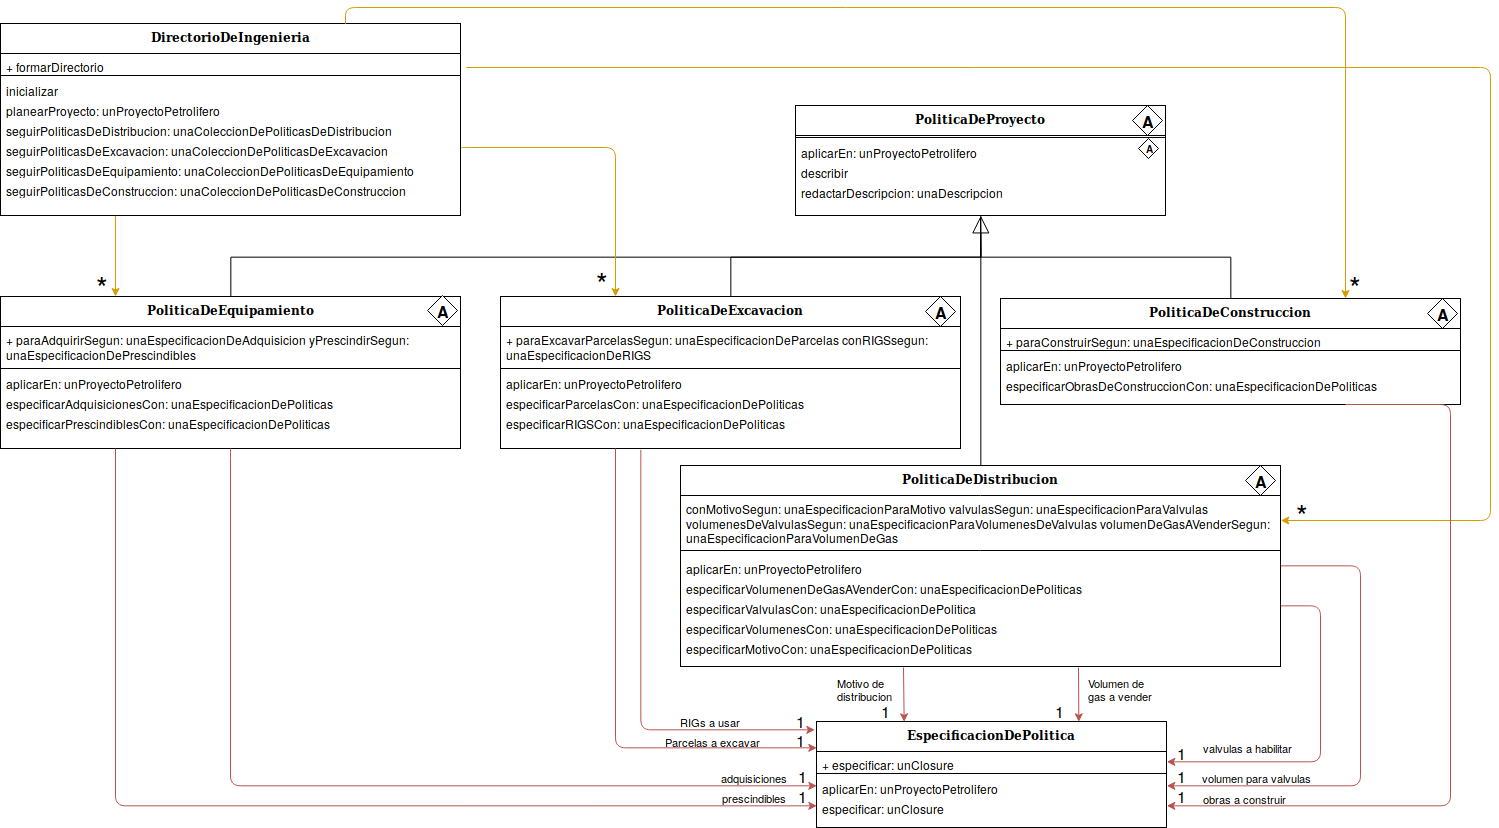
\includegraphics[scale=0.39]{images/DiagramaDeClases_deDirectorioDeIngenieria.png}}
\caption{Diagrama de clases del Directorio de Ingeniería}
\end{figure}

El directorio de ingeniería representa al equipo de ingeniería encargado de tomar todas las decisiones del día a día del proyecto, para lo cual utiliza una serie de políticas de proyecto. Para poder desempeñar esto, se le envía al comienzo de cada día el proyecto petrolífero. Una vez con esto en mano, el directorio de ingeniería para tomar sus decisiones utiliza una serie de políticas de proyecto, aplicando secuencialmente las políticas de cada tipo (permitiendo aplicar tantas como se quiera del mismo tipo). Vale aclara que para el planeamiento completo del día el directorio de ingeniería conoce políticas de distintos tipos acordes a cada sub plan del plan del día, que emplea según corresponde. Por ejemplo para documentar las decisiones de excavación en el plan de excavación se emplea únicamente las políticas de excavación.

\subsubsection{Constructora}

\begin{figure}[H]
\centerline{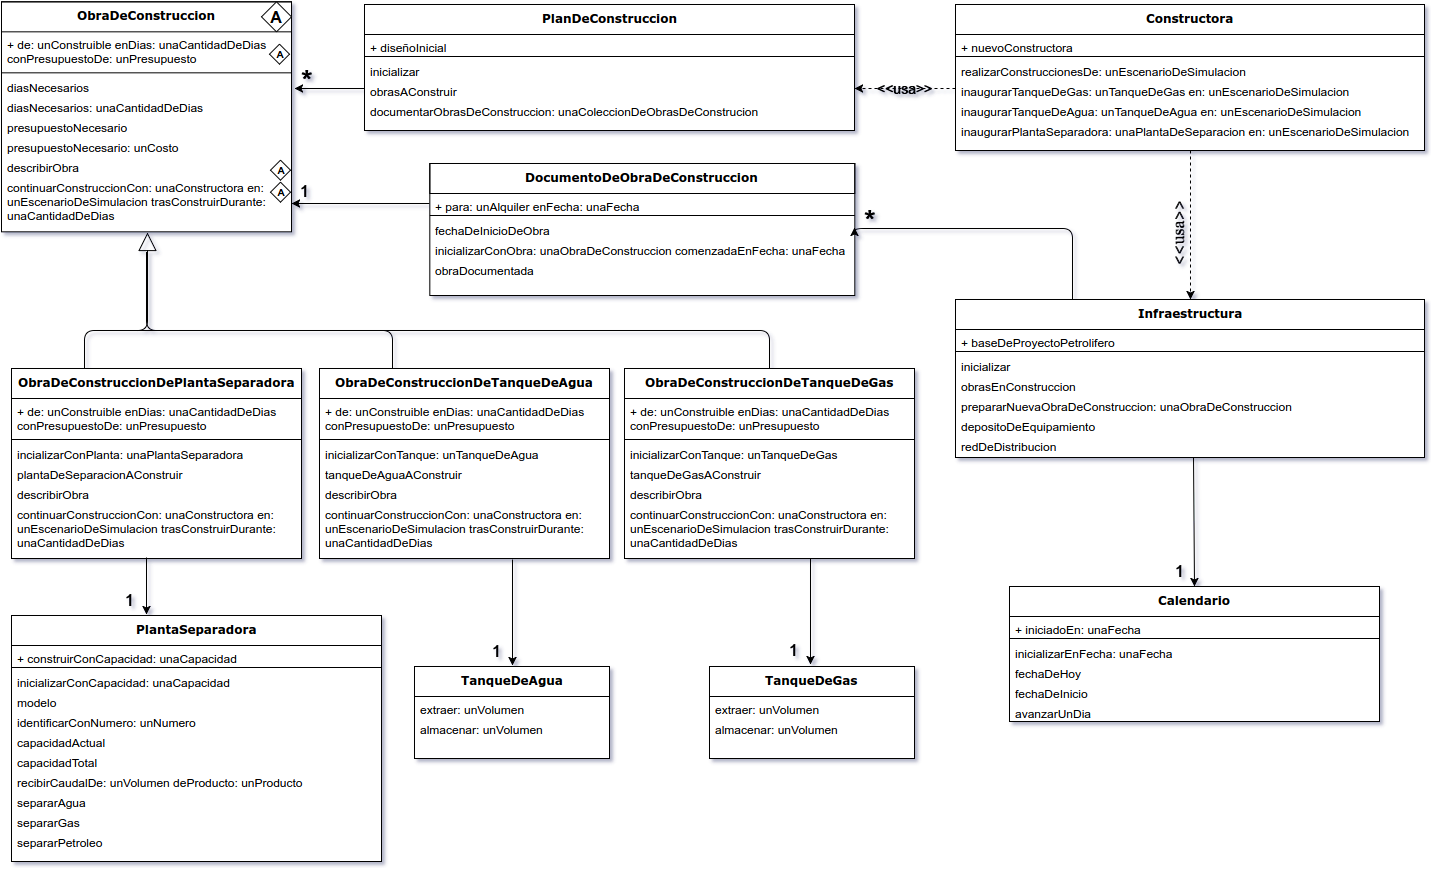
\includegraphics[scale=0.40]{images/DiagramaDeClases_deConstructora.png}}
\caption{Diagrama de clases de la Constructora}
\end{figure}

La constructora es quien se encargar de efectuar lo dictaminado con respecto al desarrollo edilicio del emprendimiento, en base a lo dictaminado previamente en el plan de construcción. En dicho plan se describe cuales son las nuevas obras de construcción que deben comenzarse. Actualmente existes tres tipos de obras de construcción, las de plantas de separación, tanques de agua, y de gas. Indiferentemente del tipo, la constructora se encarga de indicarle a la infraestructura del escenario de simulación que comience dichas obras. La infraestructura se encarga de documentar todas las nuevas obras que la constructora le despacha, con su respectiva fecha de inicio. De esta manera cada vez que la constructora le informa a la infraestructura que se debe continuar con la construcción de las obras documentadas, la infraestructura estima cuantos días pasaron desde la documentación de cada obra, y en base a eso cada obra se concluye cuando corresponda. Al concluir cada obra (cosa que se resuelve en la misma obra de construcción) esta invoca a la constructora a modo de double-dispatch, a quien le pide que le incorpore en la infraestructura, con su método de incorporación al tipo de obra en cuestión. Por ejemplo, una obra de construcción de planta separadora al darse cuenta que se concluyo, esto en base a los días necesarios, y los días ya trabajados (pasados por parámetro en el método de continuarConstruccionCon..), le envía a la constructora el mensaje de inaugurarPlantaSeparadora, quien resuelve a donde debe incorporarla. Esto por un lado desacopla la construcción de las obras del tipo de obra construido, de manera que tenemos extensibilidad por el lado de poder agregar nuevos tipos de construcción sin afectar la rutina descripta. 
  
\subsubsection{Excavador}

\begin{figure}[H]
\centerline{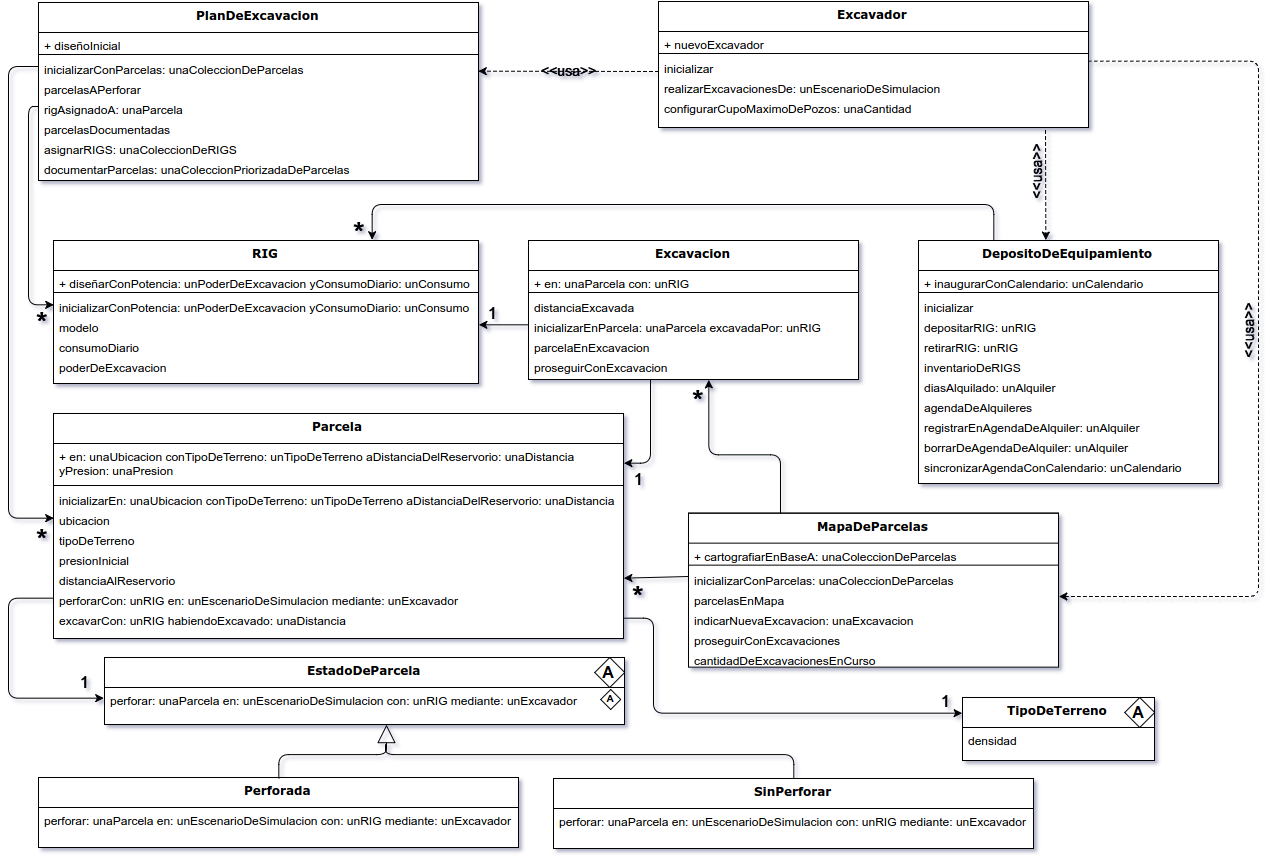
\includegraphics[scale=0.45]{images/DiagramaDeClases_deExcavador.png}}
\caption{Diagrama de clases de un Excavador}
\end{figure}

Como dijimos antes el Excavador es el que se encarga de orquestar las excavaciones a realizar en el yacimiento. Para esto va a usar el Plan de excavación para saber cuando iniciar nuevas excavaciones, ya que el Plan de Excavación es el que conoce las perforaciones pendientes; el Deposito de Equipamiento, que conoce los RIGs que están disponibles, registra sus usos y puede alquilar nuevos RIGs y los RIGs saben cuanto pueden excavar y cuanto consumen; por ultimo también usa el Mapa de Parcelas para poder realizar las excavaciones en parcelas existentes del yacimiento.

Cuando el Excavador quiera iniciar una excavación, este le dirá al Mapa para que este cree una Excavación que va a conocer el RIG que la realiza y la Parcela donde esta ubicada. Esta Excavación va a ir excavando la Parcela, la cual sabe cual es su densidad porque conoce su Tipo de Terreno (que es una clase abstracta, para hacerlo mas extensible, y se define cuando se crea el mapa de parcelas), y sabe cual es su profundidad.

Por ultimo la Parcela conoce el estado en el que esta, si esta Perforada o No, que son subclases de un Estado de Parcela. Esto sigue el patrón State para saber si se puede realizar o no un excavación, osea si ya esta perforada, al pedirle al estado que perfore este no hará nada. Es claro entender que perforar se perfora una vez, y luego se excava.

\subsubsection{Fletador}

\begin{figure}[H]
\centerline{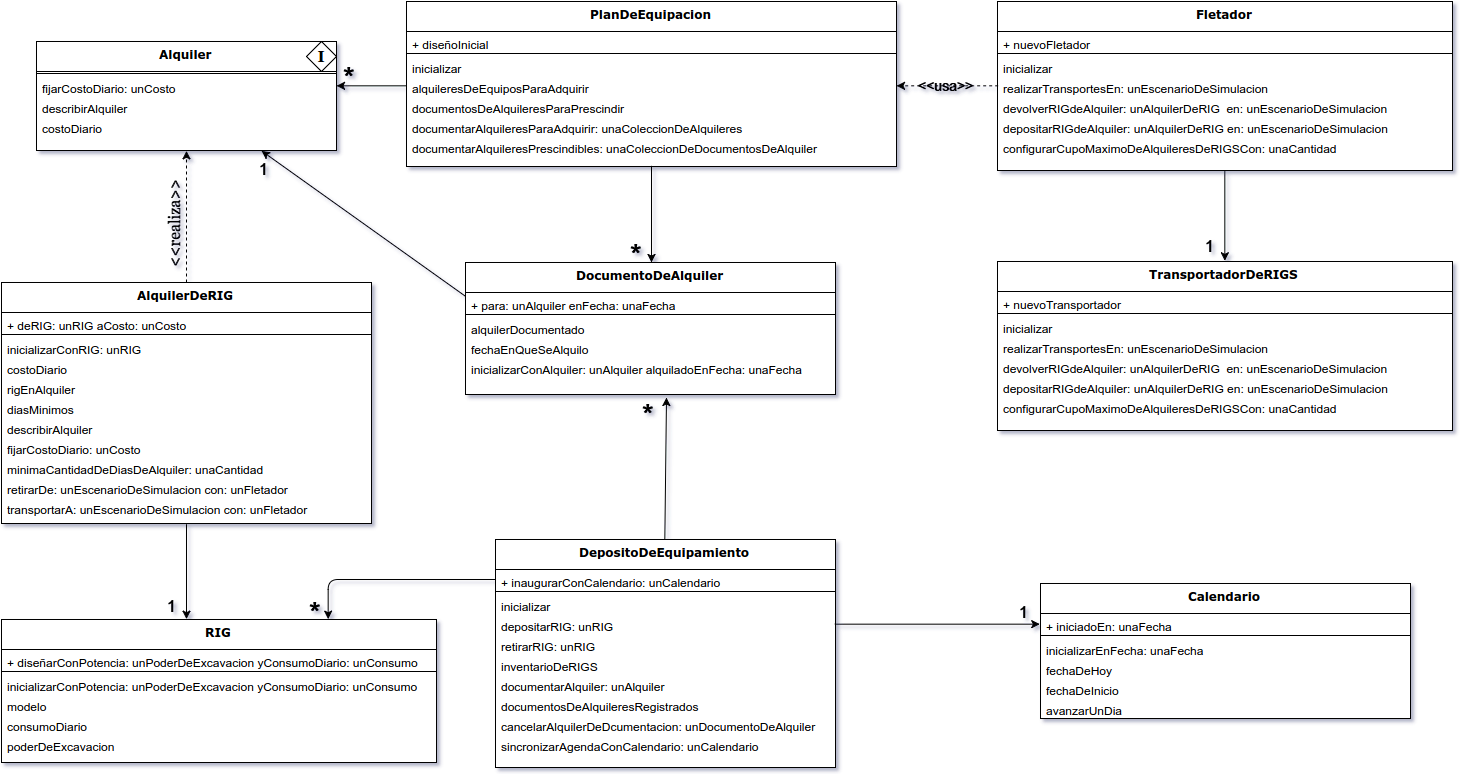
\includegraphics[scale=0.38]{images/DiagramaDeClases_deFletador.png}}
\caption{Diagrama de clases de un Fletador}
\end{figure}

El Fletador se encarga de realizar todos los despachos del equipamiento del emprendimiento. Con equipamiento nos referimos a cualquier tipo de maquinaria o recursos no edilicios (o construibles por una obra). Para esto la idea con respecto al Fletador es que conozca otro objeto con una dedicación mas especifica sobre el despacho de un cierto equipamiento, en nuestro caso el TransportadorDeRIGs. Esto forma parte del enfoque de extensibilidad y de modularidad del diseño, ya que al tener varias clases con dedicación mas particular es mas fácil de modificar en caso de un nuevo requerimiento, sin impactar a otros objetos. En nuestro caso particular el único tipo de equipamiento que hay son los RIGs, por lo que podríamos simplemente tener solo al Fletador.

A la hora de realizar los transportes del equipamiento, el Fletador se debe encargar de la parte administrativa de los mismo. Con esto nos referimos a garantizar que los alquileres sean documentados en el deposito. De manera que en caso de depositarlo, pedir que el alquiler depositado se documente; y en caso de retiro del equipo, que se pida cancelar su respectiva documentación. La documentación en este sentido actúa como un contrato en que se estampa la fecha de la toma del alquiler, y sirve además para que al momento de querer cancelar dicho alquiler, se verifique contra la fecha de toma del alquiler para saber si se cumplió el plazo mínimo de días en alquiler.

Vale aclarar que la razón por la que modelamos una interfaz Alquiler es mas que nada para mostrar la idea de que los documentos de alquiler es que conozcan cualquier tipo de alquiler posible, si es que se desea extender el sistema para que soporte otros tipos de alquileres. Podríamos haberla modelado también como una clase abstracta, pero no queríamos incurrir a la subclasificación sin ser requerida en base a los principios de diseño visto en clase.


\subsubsection{AdministradorFinanciero}

\begin{figure}[H]
\centerline{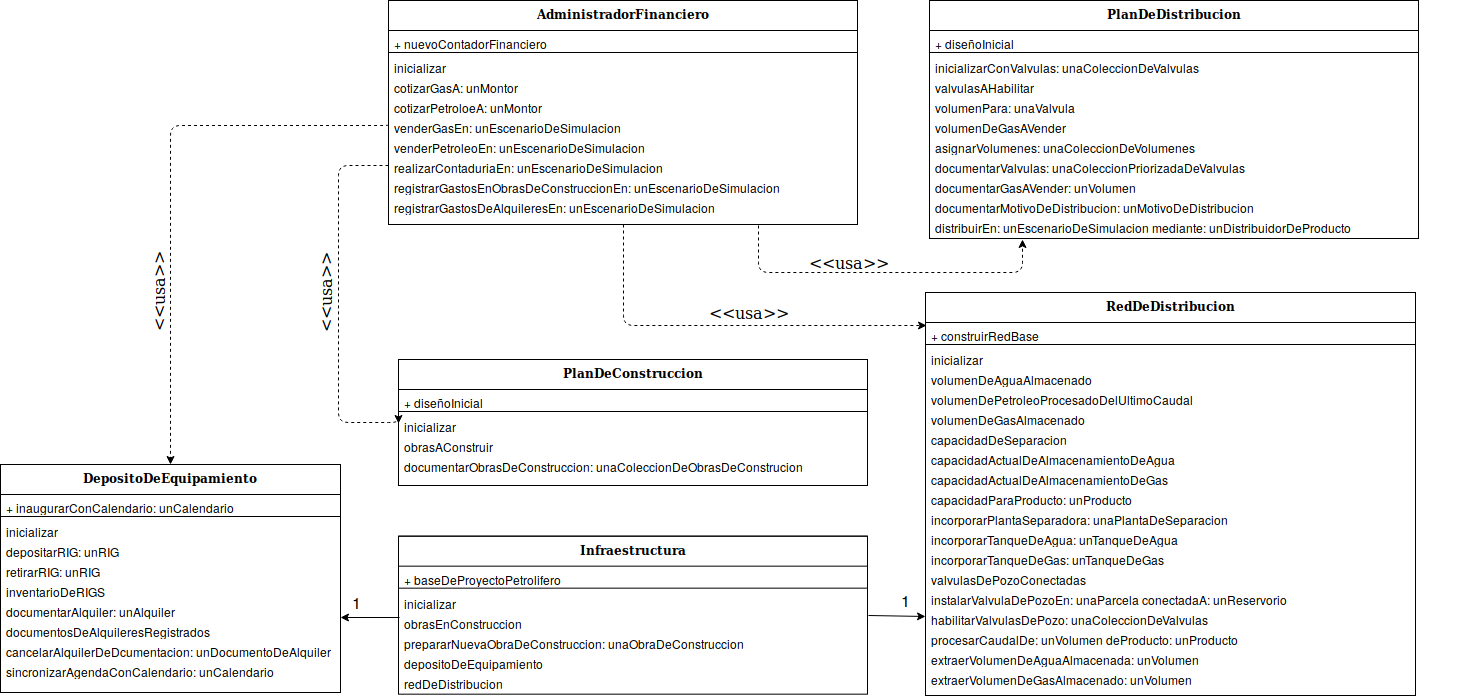
\includegraphics[scale=0.38]{images/DiagramaDeClases_deAdministradorFinanciero.png}}
\caption{Diagrama de clases de un AdministradorFinanciero}
\end{figure}

El Administrador financiero se encarga de realizar las estimaciones de contaduría del día, y registrarlos en el registro de contaduría. Hay 4 tipos de factores a tener en cuenta para ello, el primero son las obras de construcciones que se mandaron a construir en ese, para ello consulta el plan de construcción del día en el que se han dictaminado, vale aclarar que a diferencia de los alquileres, asumimos que las obras de construcción siempre se pagan totalmente el mismo día de su inicio. Otro factor son los gastos de alquileres que se deben ir cobrando día a día, para ello el Administrador financiero consulta todos los documentos de alquiler registrados en el deposito, para obtener el costo de cada uno (este es cobrado mas allá de si el RIG se esta utilizando actualmente en una excavación o no). Finalmente pero no menos importante, el Administrador financiero consulta el volumen de petroleo procesado, para luego estimar la ganancia en base a la cotización de petroleo configurada, análogamente se calcula el volumen de gas extraído y se estima su ganancia también con la catalicón de gas. A diferencia del petroleo, en este caso el Administrador financiero debe extraer de la red de distribución el volumen dictaminado en el plan de distribución. Debido a que esto esta dictaminado en el plan de distribución pensamos que la parte de extracción de lo anterior debería hacerlo el Extractor, en vez del Administrador financiero 

\pagebreak

\subsubsection{Registradores}

\begin{figure}[H]
\centerline{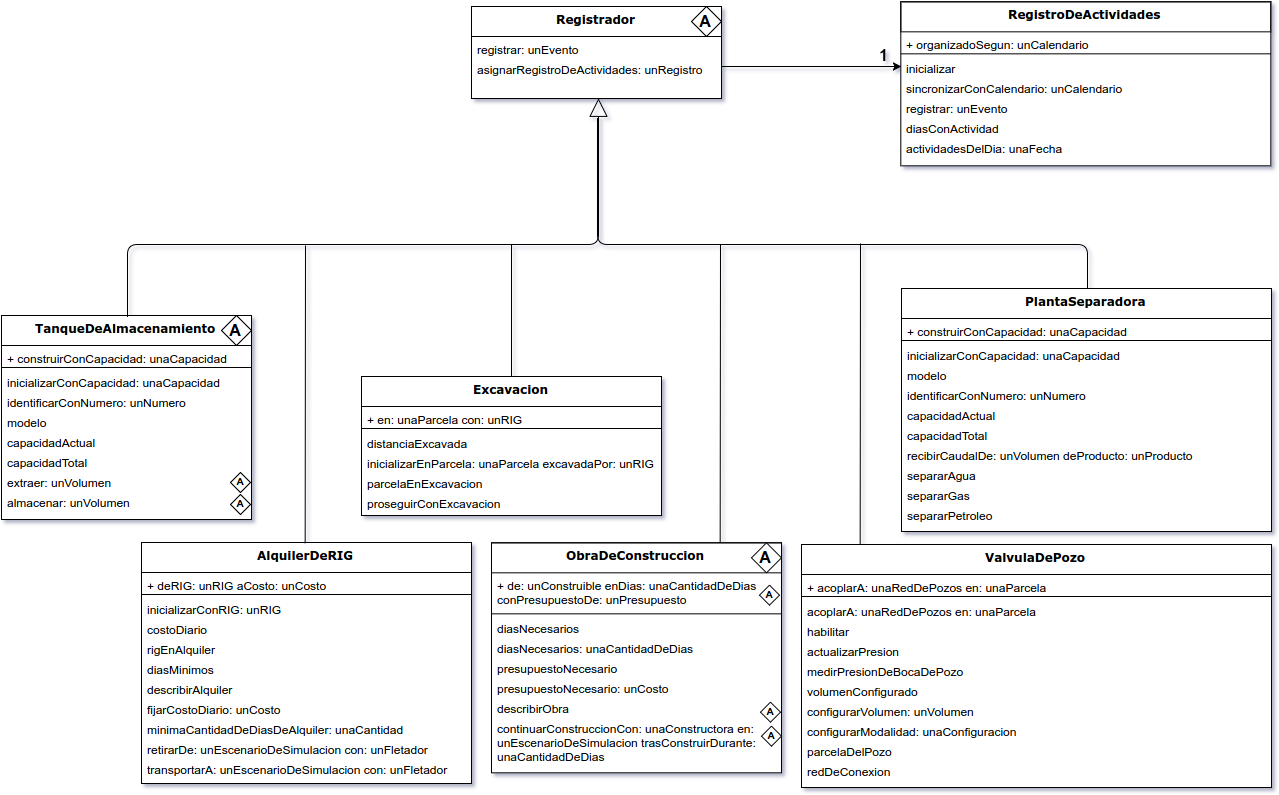
\includegraphics[scale=0.44]{images/DiagramaDeClases_deRegistrador.png}}
\caption{Diagrama de clases de Registradores}
\end{figure}

  Dado que necesitábamos registrar actividades muy diversas del emprendimiento, decidimos determinar cierto objetos que hagan de testigos (o registradores) de dichas actividades. Para esto utilizamos un patrón observer, haciendo que dichos testigos, determinados por ser subclases de la clase Registrador, registren los eventos registrados en algún registro asignado. Nos pareció que los mas adecuados eran:
  
  \begin{itemize}
  
  \item ObraDeConstruccion: Registra cuando se empezó a construir una obra de ese tipo, y a mediado que se continua la obra día a día, cuantos días faltan, como así también cuando se concluyo la obra. 
  
  \item AlquilerDeRIG: Registra cuando se tomo dicho alquiler.
  
  \item ValvulaDePozo: Registra si se extrajo o reinyecto de alguna forma por medio de ella y cuanto volumen dejo pasar.
  
  \item Excavacion: Registra cuanto se excavo en su respectiva parcela, identificándola por su ubicación.
  
  \item TanqueDeAlmacenamiento: Registra el volumen que se almacena o extrae del mismo.
  
  \item PLantaSeparadora: Registra el volumen de agua, gas y petroleo que se separa de la misma.

  \end{itemize}
  
  Dado que cada uno de estos objetos testigos implementan su propia forma de registrar, el agregar nuevos objetos que deben registrar no impacta en el funcionamiento e implementación de los registradores preexistentes.

\pagebreak

\subsubsection{Distribuidor}

\begin{figure}[H]
\centerline{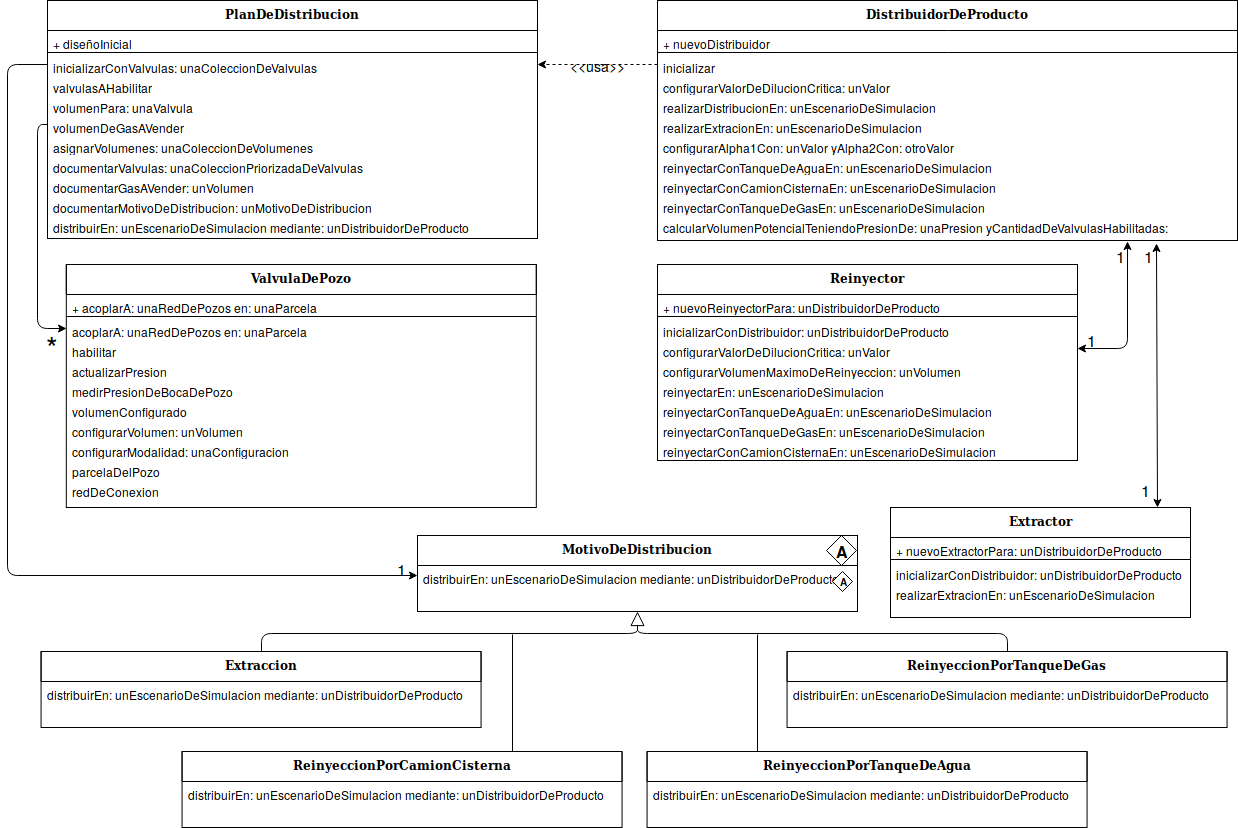
\includegraphics[scale=0.44]{images/DiagramaDeClases_deDistribuidor.png}}
\caption{Diagrama de clases del Distribuidor}
\end{figure}

El distribuidor es el encargado de realizar la distribución del día a día. Hablamos de distribución cuando nos referimos al volumen de líquidos distribuidos por la red de distribución. Para determinar como se quiere distribuir durante el día de hoy, el distribuidor consulta el plan de distribución al que se le indica que se quiere distribuir. En consecuencia el plan reenvia el mensaje al MotivoDeDistribucion, junto con el escenario de simulador y el distribuidor que le habían pasado. Este motivo puede ser Extracción, ReinyeccionPorTanqueDeAgua, ReinyectorPorTanqueDeGas, o ReinyeccionPorCamionCisterna, según cual sea enviada un mensaje acorde al distribuidor sobre que hacer. El distribuidor en consecuencia despacha la responsabilidad al Reinyector o al Extractor según corresponda y luego procederán a configurar y mandar a habilitar las válvulas.

\pagebreak

\subsection{Diagramas de secuencias/colaboración}

Los diagramas aquí presentes se encuentran disponibles en tamaños considerablemente mas grandes en el Anexo.

\subsubsection{Planear Proyecto}

\centerline{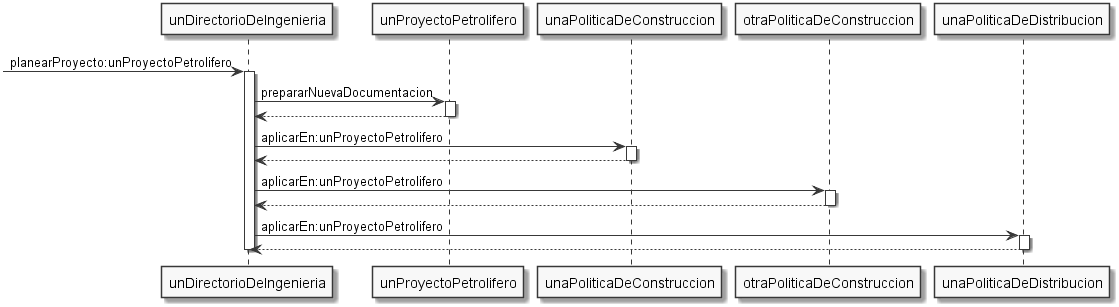
\includegraphics[scale=0.45]{images/secuenciaPlanearProyecto1.png}}
\vspace{0.25cm}
\centerline{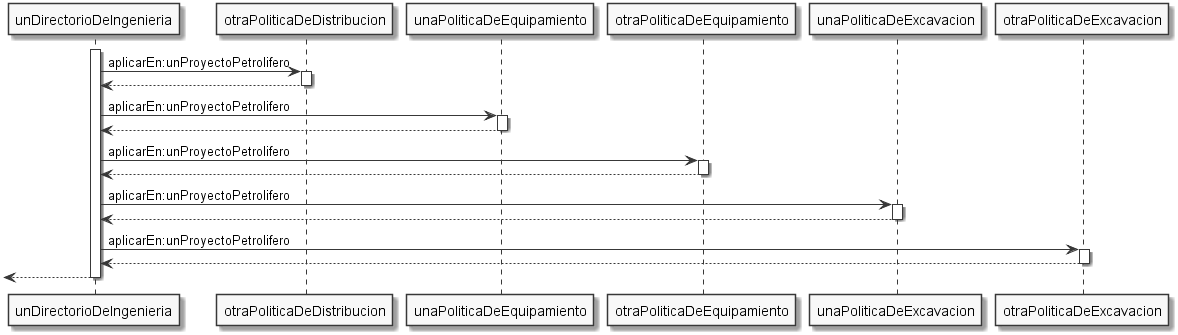
\includegraphics[scale=0.45]{images/secuenciaPlanearProyecto2.png}}

En este diagrama podemos ver como se realiza la planificación de un proyecto, primero se prepara una nueva documentación del día, esto nos da una serie de políticas base, y nos da la posibilidad de agregar nuevas políticas. Luego se aplican varias políticas nuevas, estas se agendan en la documentación que preparamos anteriormente.

\subsubsection{Construcción}
\centerline{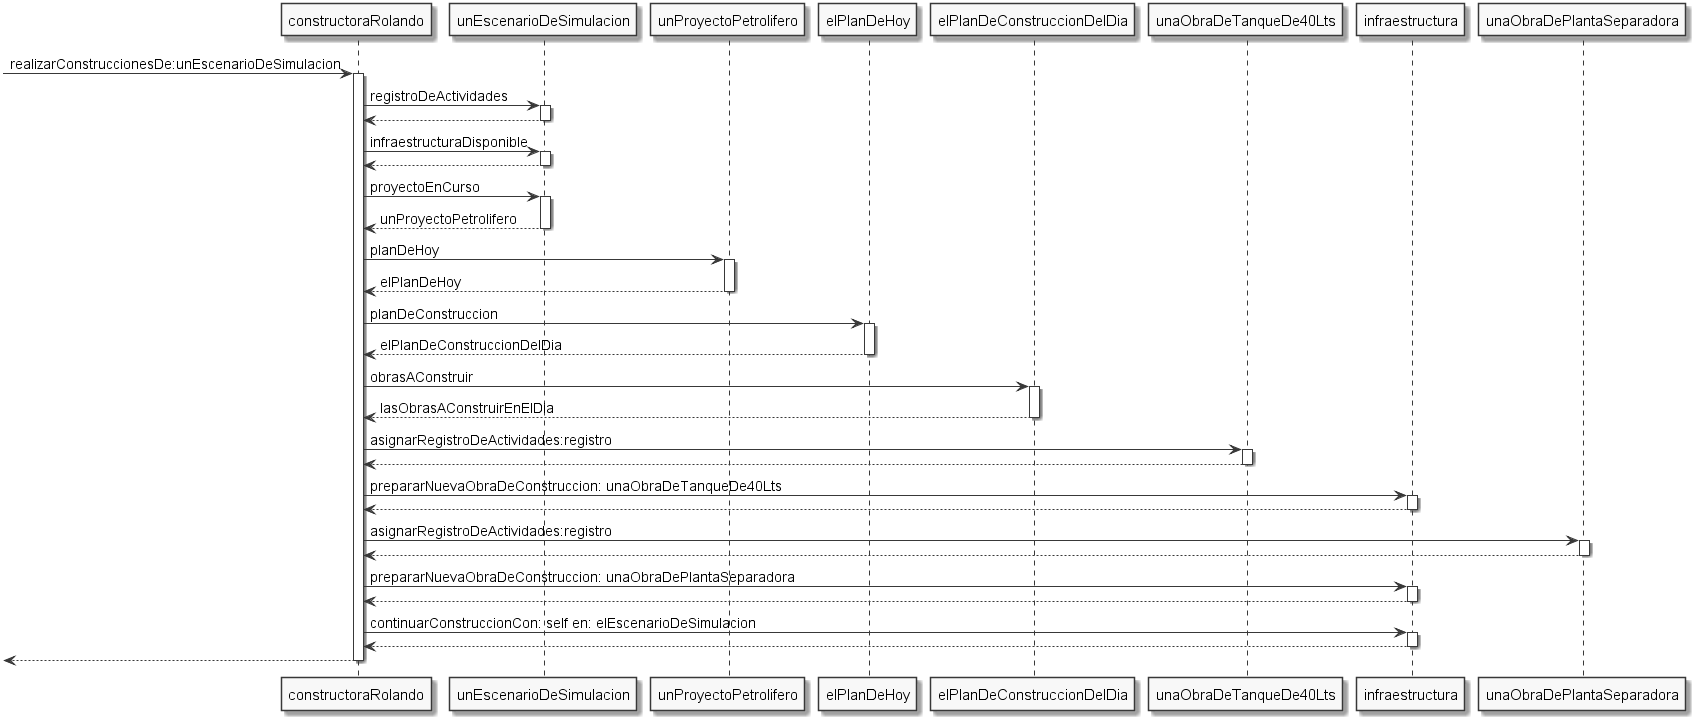
\includegraphics[scale=0.325]{images/secuenciaConstruir.png}}
\vspace{0.25cm}
\centerline{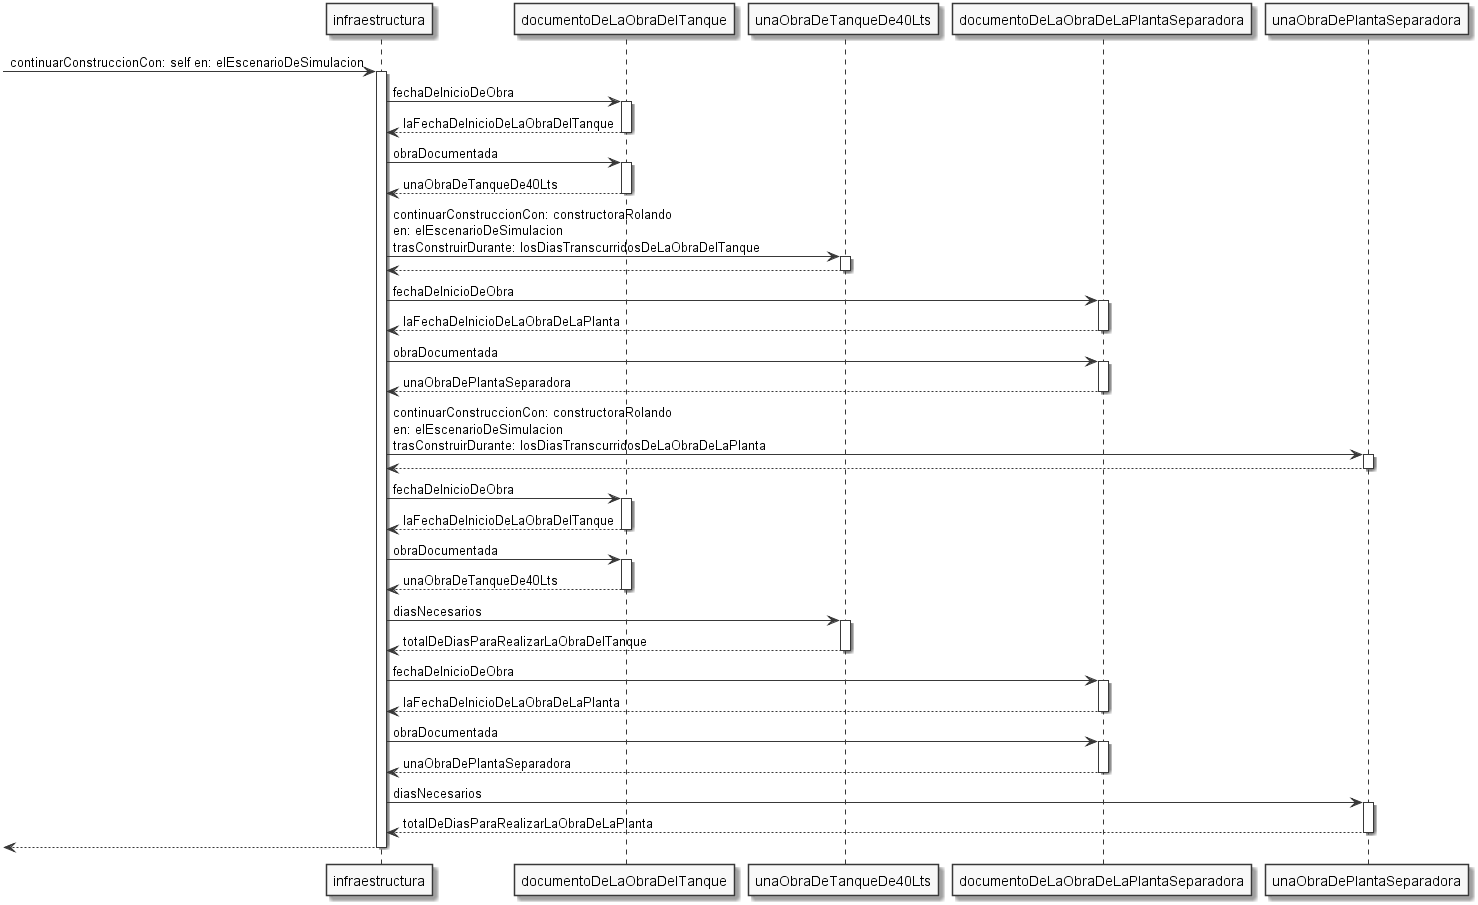
\includegraphics[scale=0.325]{images/secuenciaConstruirInfraestructura.png}}

El primer diagrama nos muestra como se aplican las políticas de construcción, particularmente vemos como se agregan dos nuevas obras de construcción al yacimiento, estas son un tanque de 40Lts y una planta separadora, estas obras se preparan y se agregan al registro. Posteriormente, se comienza con las construcciones del días, para hacer esto se hace un double-dispatch hacia la infraestructura con la constructora.

El segundo diagrama muestra como se continua con las construcciones en el día, la encargada de enviar la constructora a la obra es la infraestructura. La obra recibe a la empresa constructora, junto con los días transcurridos de la construcción, en caso de que se alcancen los días necesarios para completar la construcción de la obra, la misma le indica a la infraestructura se ha completado. Si no se completo la obra, se actualiza la cantidad de días necesarios para completar la misma.

\subsubsection{Distribución}

\centerline{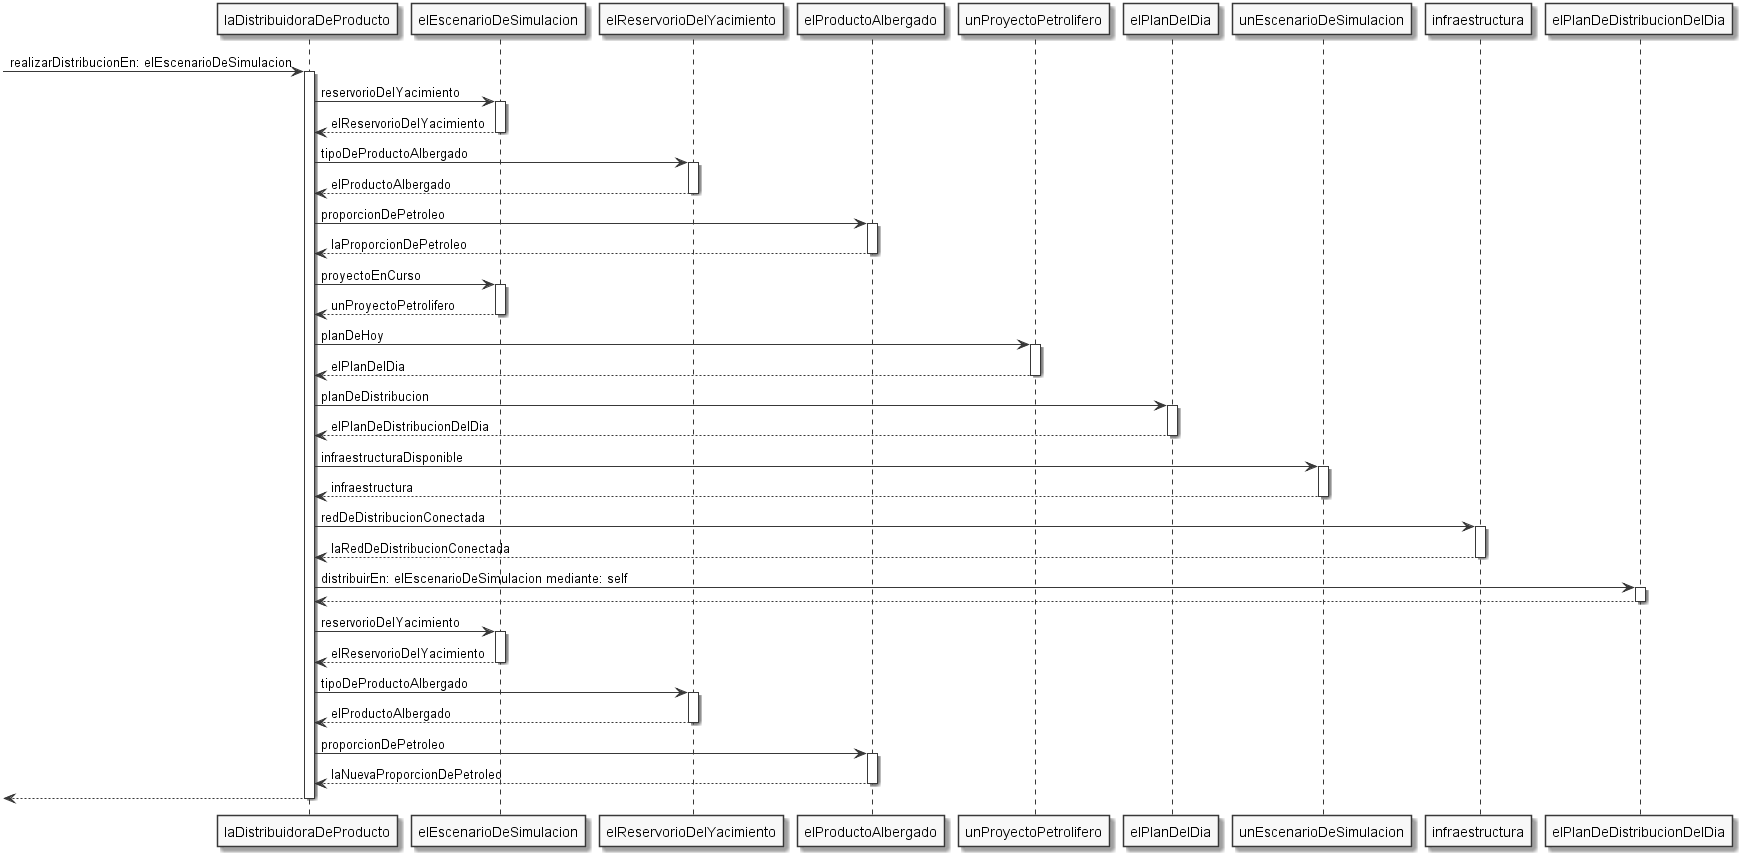
\includegraphics[scale=0.325]{images/secuenciaDistribucion.png}}

Este es el primer diagrama que muestra la distribución, en este primer paso se analiza la proporción de petroleo del reservorio, si esta no es menor a la proporción critica no se procede con la políticas de distribución. En caso de que la proporción sea adecuada, se procede con las políticas de distribución, y luego se procede a calcula la nueva proporción de petroleo en el reservorio.

\subsubsection{Distribución: Extracción}

\centerline{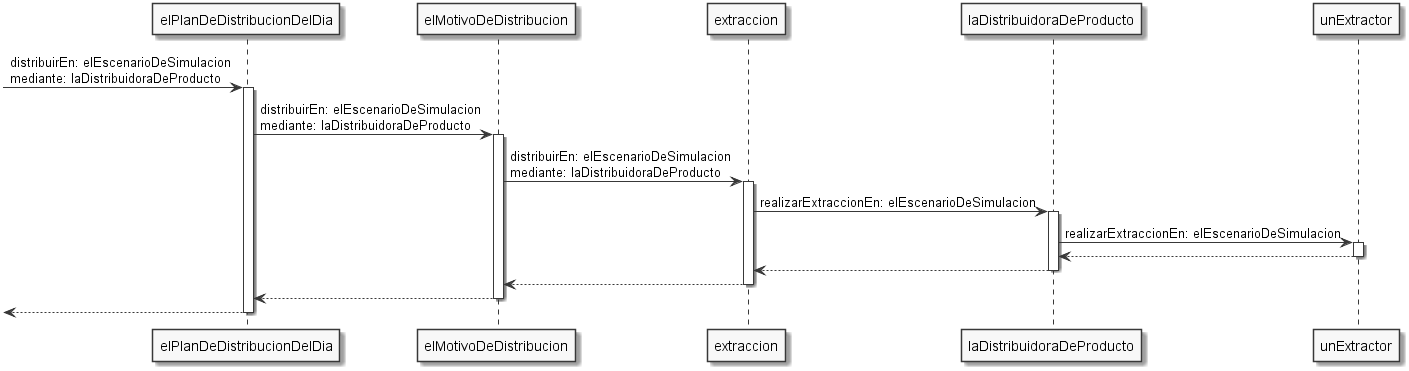
\includegraphics[scale=0.325]{images/secuenciaDistribucionMotivo1.png}}
\vspace{0.25cm}
\centerline{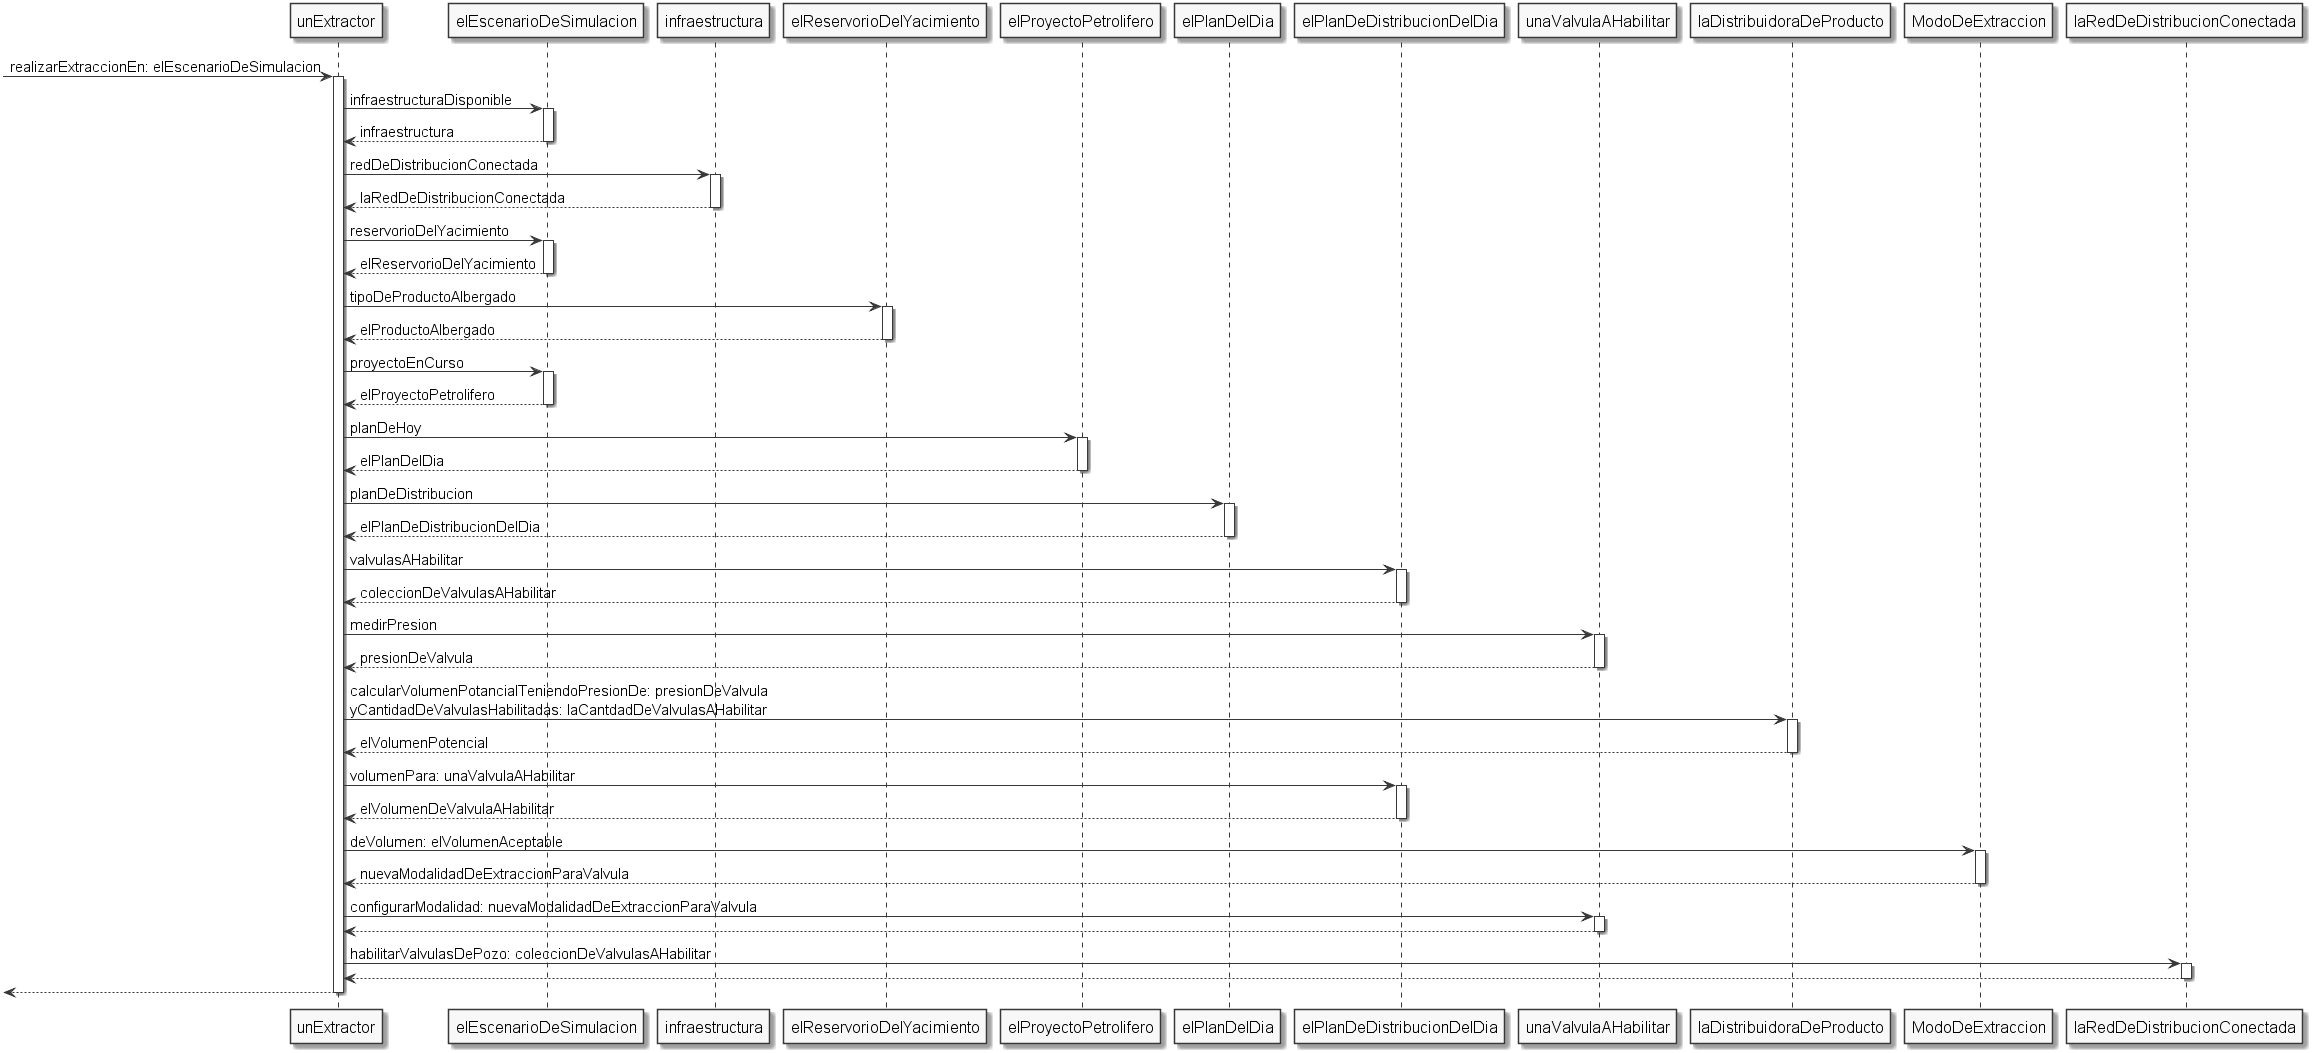
\includegraphics[scale=0.2]{images/secuenciaDistribucionMotivo2.png}}

Este caso muestra la aplicación de un política de distribución, acá el Motivo de Distribución es una extracción, el cual le comunica a la Distribuidora de Producto que le indica al Extractor que puede realizar el proceso de extracción. Para todas las válvulas que se desean habilitar para la extracción, se calcula el volumen potencial para la extracción, y luego con esto se calcula el volumen aceptable, el cual establece la modalidad de extracción que indica cuanto se desea extraer de cada válvula. Este proceso se repite para todas las válvulas, una vez que todas las modalidades se establecieron, se procede a habilitar las válvulas elegidas.

\subsubsection{Distribución: Reinyección con Tanque de Agua}

\centerline{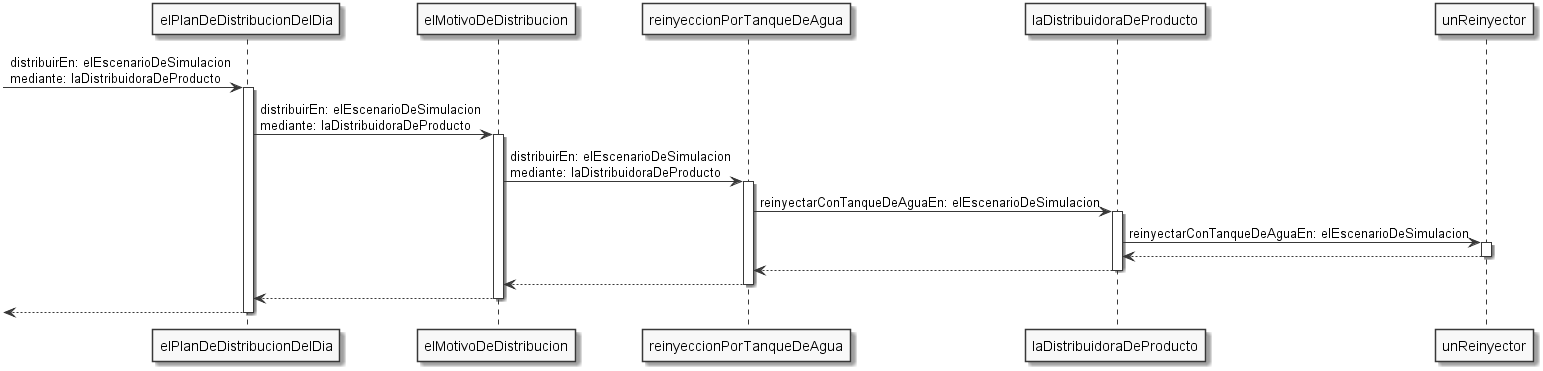
\includegraphics[scale=0.35]{images/secuenciaDistribucionMotivoAgua1.png}}
\vspace{0.25cm}
\centerline{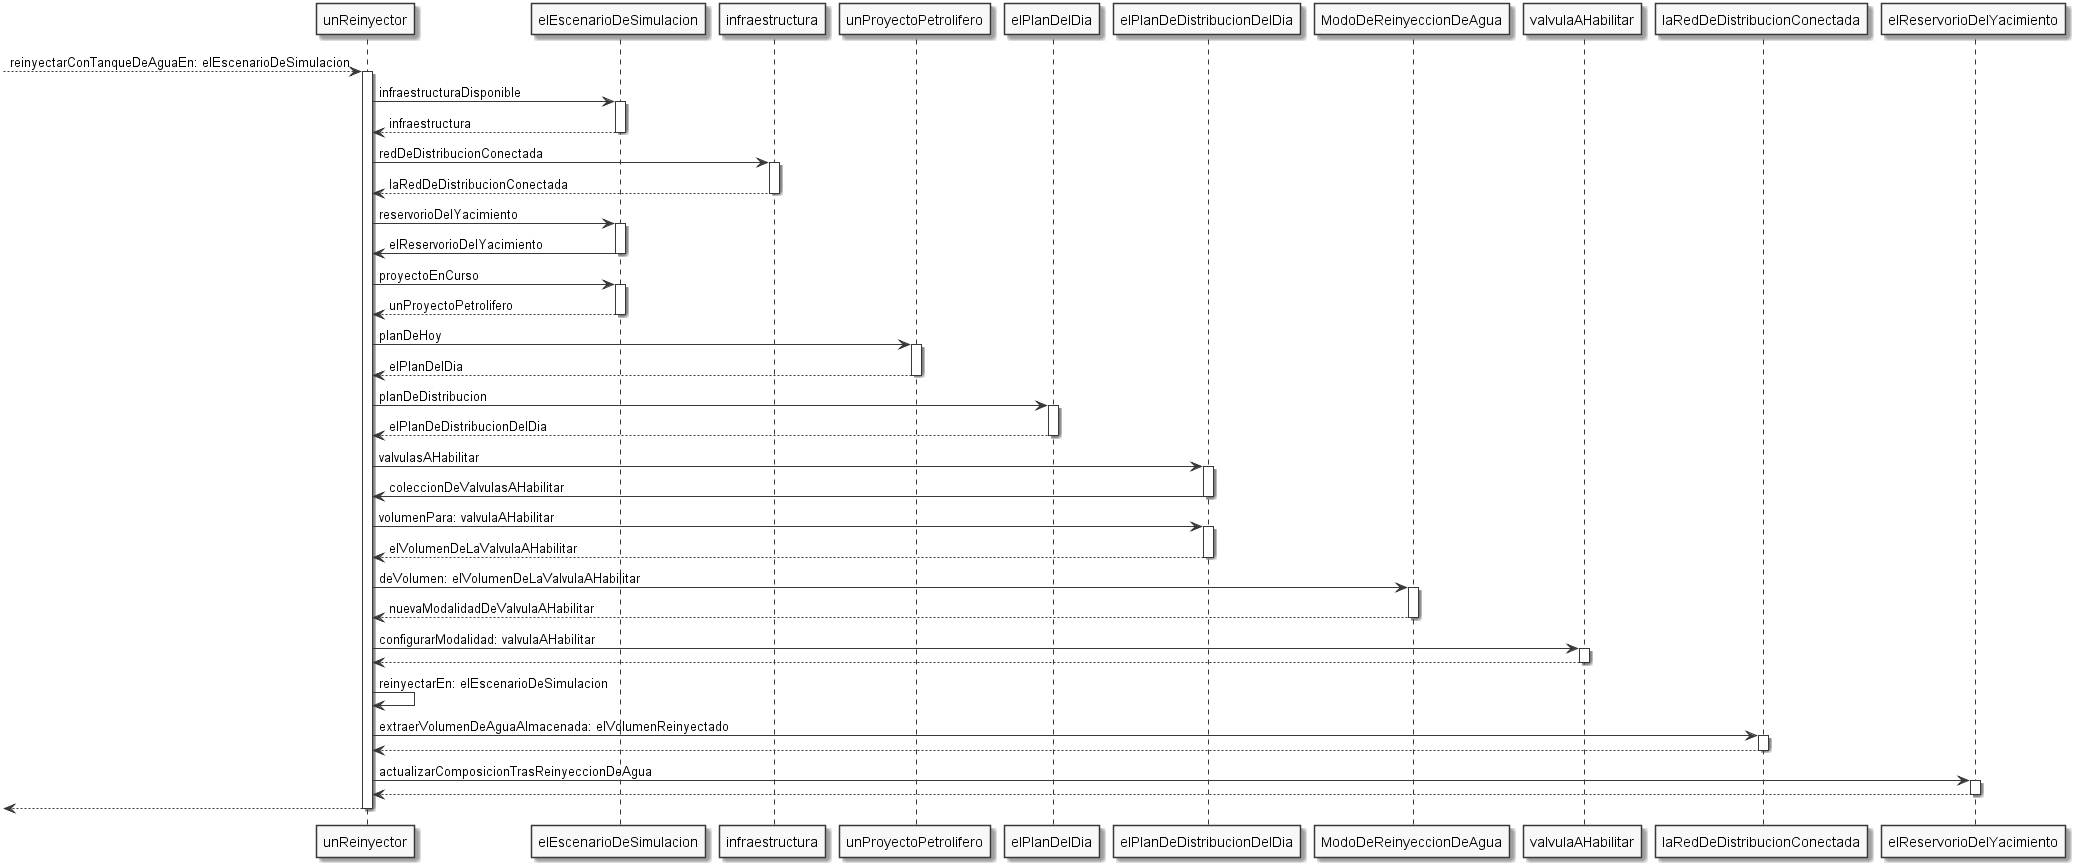
\includegraphics[scale=0.2]{images/secuenciaDistribucionMotivoAgua2.png}}

En este caso el Motivo de Distribución es una reinyección de agua con tanque, el cual le comunica a la Distribuidora de Producto que le indica al Reinyector que proceda con la reinyección de agua. El proceso es casi idéntico a la extracción, con la diferencia que la modalidad de reinyección establece cuanto se reinyecta en el pozo, esto se repite para cada uno. Una vez concluido el proceso, se actualiza la cantidad de agua disponible en los tanques, y se actualiza la composición del reservorio.

\subsubsection{Equipamiento}

\centerline{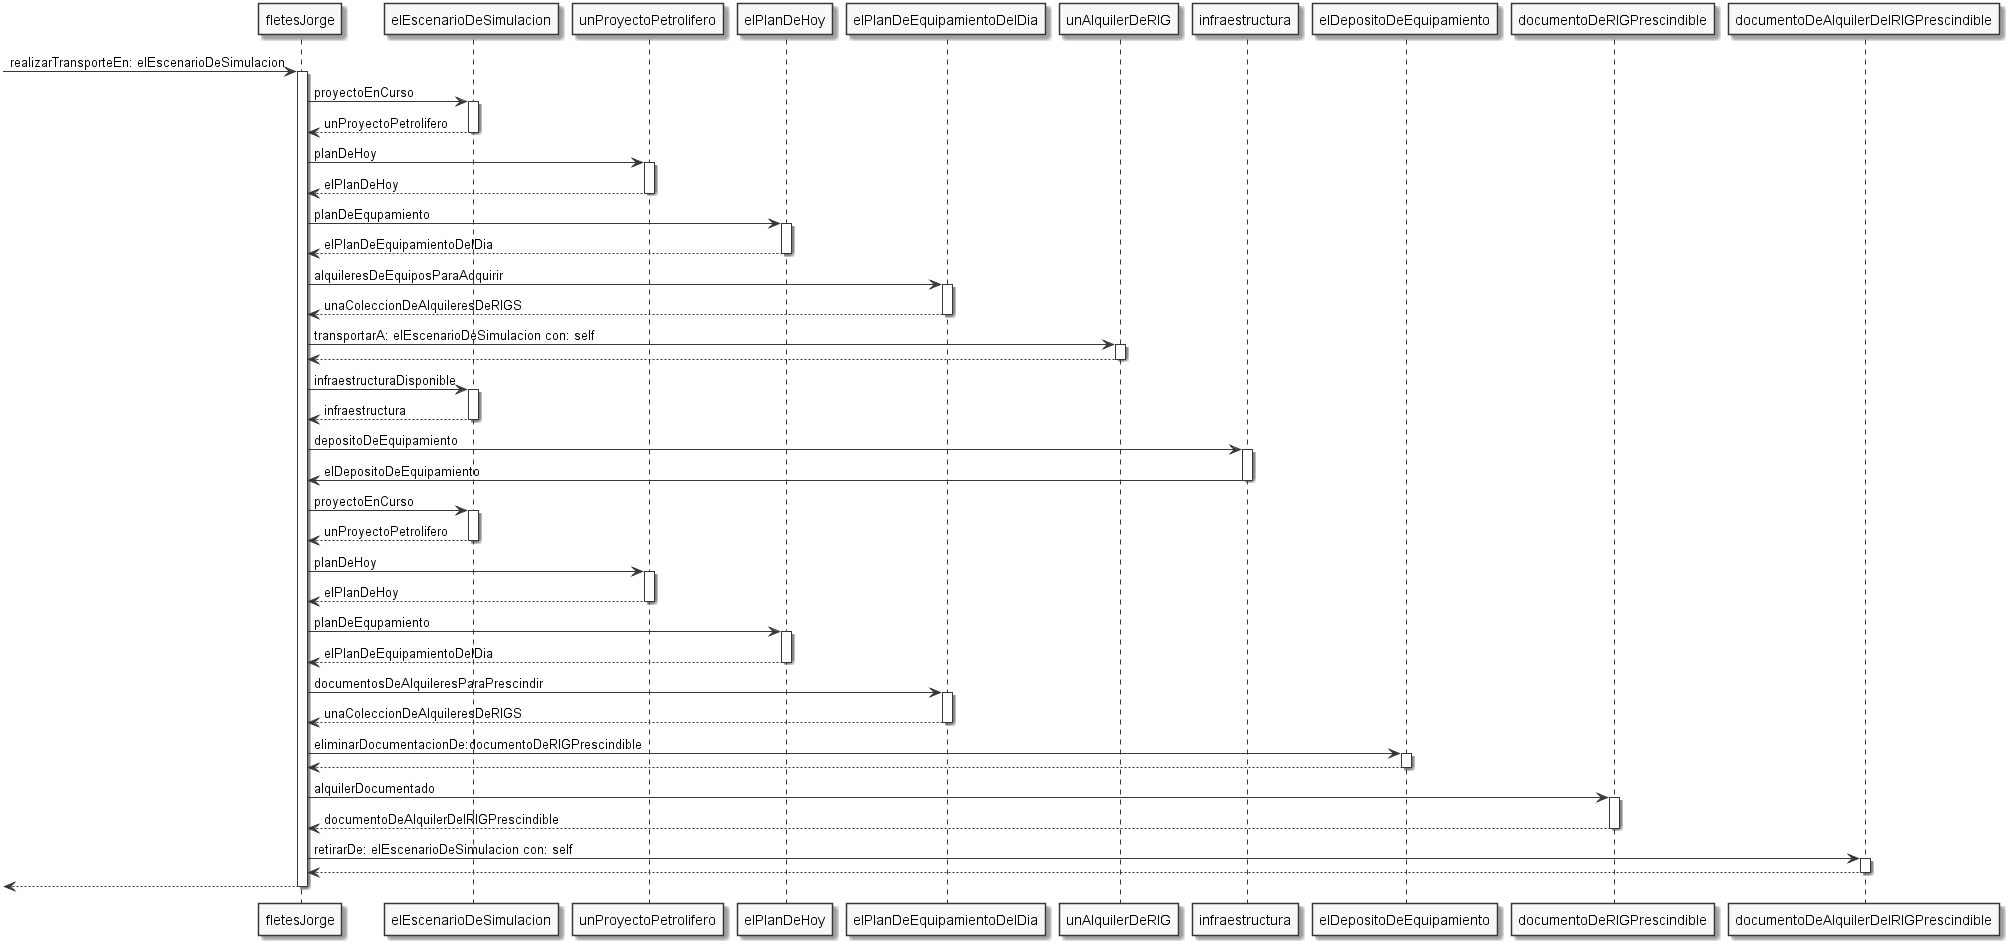
\includegraphics[scale=0.25]{images/secuenciaEquipamiento.png}}
\vspace{0.25cm}
\centerline{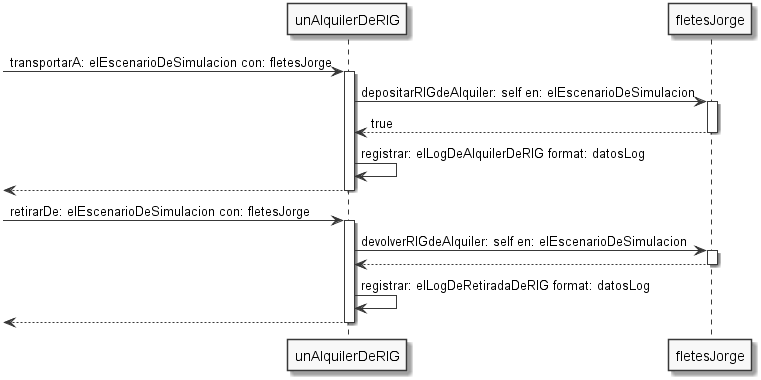
\includegraphics[scale=0.5]{images/secuenciaEquipamientoTransportar.png}}

En el primer diagrama podemos ver como se aplica una política de equipamiento, la misma dicta que equipos alquilar y de que equipos se ha concluido el periodo de alquiler y no se ha renovado el mismo. Para cada equipo que se desea alquilar se arma un documento de alquiler, luego la compañía de fletes se encarga de traerlo al deposito, y procede a comunicarle al escenario de simulación que el mismo ha sido depositado junto con el documento de alquiler. Para aquellos equipos cuyo alquiler se ha vencido, se envía a la compañía de fletes para que remueva el mismo del sistema. Tanto como para pedir el alquiler, depositar y retirar a un equipo se utilizo el mismo documento de alquiler, este deja de existir únicamente cuando el equipo finalmente es retirado del yacimiento.

\subsubsection{Excavación}

\centerline{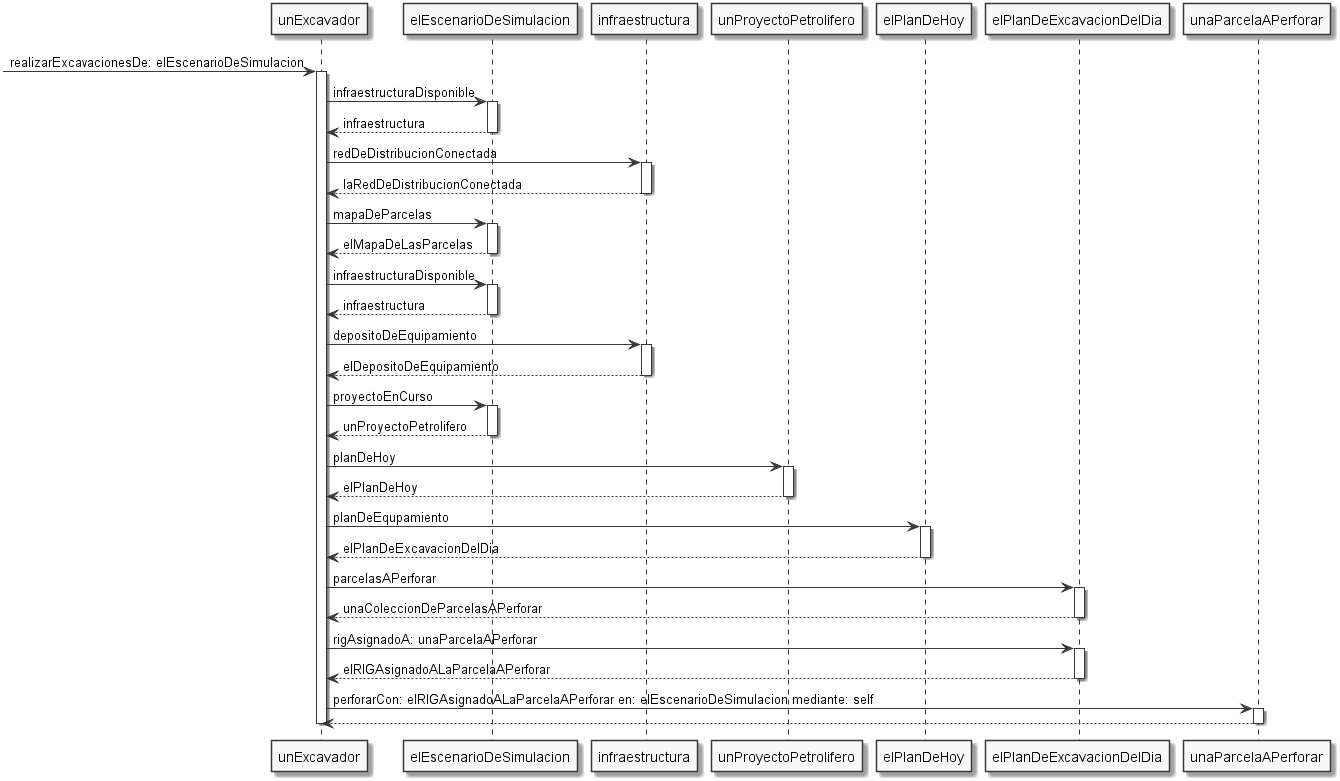
\includegraphics[scale=0.325]{images/secuenciaExcavacion1.png}}
\vspace{0.25cm}
\centerline{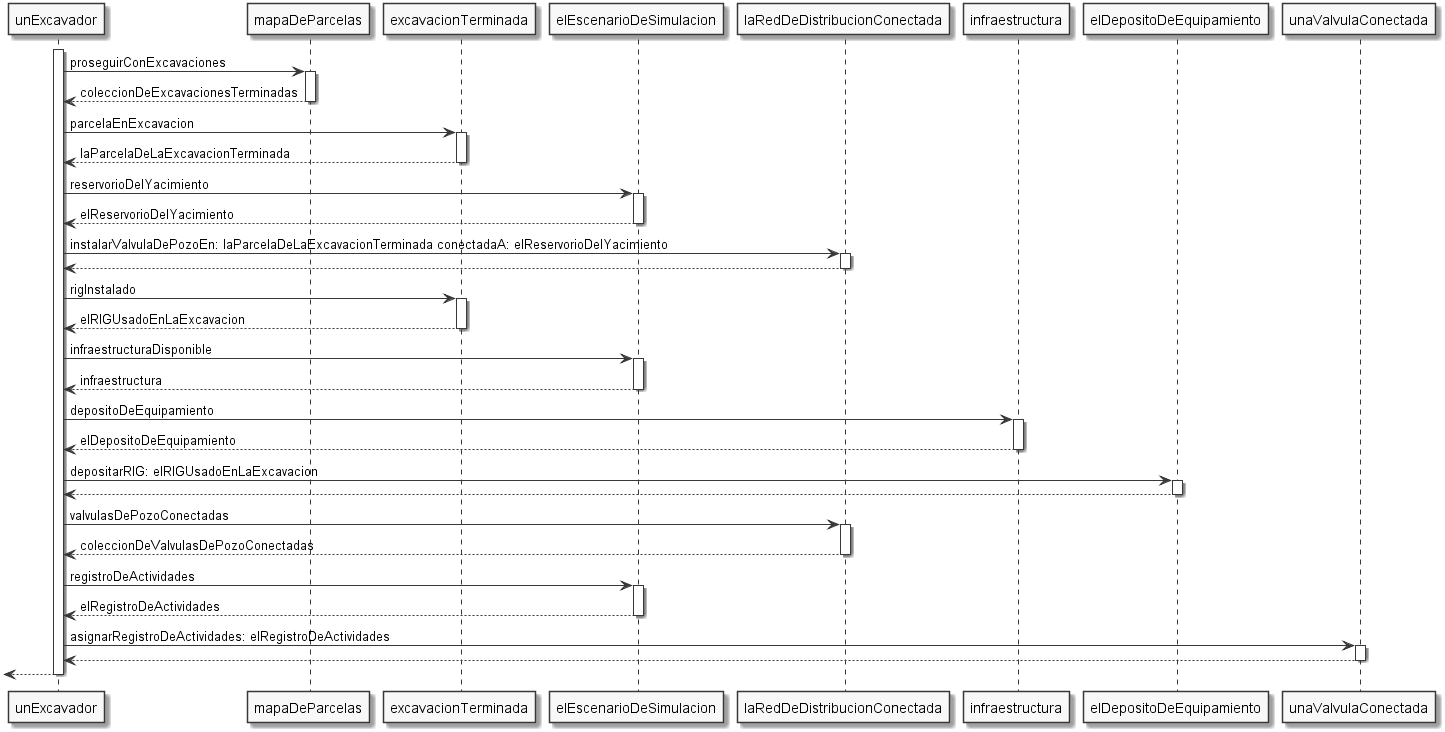
\includegraphics[scale=0.325]{images/secuenciaExcavacion2.png}}

El Plan de Excavación del día dicta en que parcelas se desean excavar, para hacer esto el Plan tiene una colección de parcelas a excavar, junto con los RIGs que han sido asignados a las mismas. Esto consiste en tomar el RIG asignado del deposito, llevar el mismo hacia la parcela asignada, instalarlo y luego conectar la válvula del mismo a la Red de Distribución del yacimiento. Una vez concluida la instalación se actualiza el deposito para indicar que el RIG utilizado en la parcela no se encuentra mas en el mismo, y se guarda el registro de las excavaciones en el registro de actividades.

\pagebreak

\section{Conclusión}

Durante el trabajo nos encontramos con varias problemáticas a resolver, a nivel diseño, especificación e implementación. Dado que la elicitación de requerimientos ya estaba bastante avanzada, consideramos que el desafió mas grande estuvo en hacer un diseño que fuese estrictamente de objetos, y a su vez que el mismo se pudiese adaptar a cambios en la especificación del problema. Intentamos evitar el uso de construcciones que en general están asociadas a lenguajes imperativos como el uso de condicionales, buscando utilizar las herramientas que proveen los lenguajes estrictamente orientados a objetos como el polimorfismo de objetos y el uso de clausuras. A su vez, buscamos un diseño con objetos cohesivos y con bajo acoplamiento, con nombres de objetos que fuesen descriptivos y con la mayor semántica posible. A grandes rasgos, consideramos que seguimos las heurísticas de diseño de objetos que estudiamos.

En el proceso de este trabajo, estudiar las diferentes metodologías de desarrollo disponibles también fue muy interesante. Ya esta ampliamente estudiado el hecho de que un proceso en cascada no lleva a buenos resultados, principalmente debido a que los requerimientos funcionales pueden cambiar, no solo debido a que el cliente puede requerir un cambio, si no que también debido a que el proceso de desarrollo lleva a un aprendizaje sobre el problema. Por otro lado, los modelos iterativos e incrementales tienen la ventaja de que el usuario ve el progreso del proyecto rápidamente. Mediante ciclos de desarrollo, a partir del feedback del cliente van cambiando los requerimientos. Existen muchas variaciones de esta metodología, como las de desarrollo Ágil. Entre ellas se encuentra SCRUM que es la que utilizamos principalmente en este trabajo.

Como reflexión final, debemos decir que al intentar respetar los principios de diseño de forma estricta, el diagrama de clases que realizamos termino siendo sumamente cargado y complejo. Es sumamente complejo realizar un diseño que sea extensible. Muchas veces quizás es mejor buscar un diseño con una semántica mejor aunque no respete algunos de estos principios.

\end{document}